% rasti_template.tex 
%
% LaTeX template for creating an RASTI paper
%
% v1.2 released 26 April 2022
% (version numbers match those of rasti.cls)
%
% Copyright (C) Royal Astronomical Society 2022
% Authors:
% Peter Jones (OUP, adapted from mnras_template.tex, author Keith T. Smith (Royal Astronomical Society))

% Change log
%
% v1.0 November 2021
%    Adapted from mnras_template.tex
% v1.1 February 2022
%    rasti.bst updated to match output style for Geophysical Journal International 
% v.1.2 April 2022
%    minor updates to author instructions (word limit, contact adddress, keywords)


%%%%%%%%%%%%%%%%%%%%%%%%%%%%%%%%%%%%%%%%%%%%%%%%%%
% Basic setup. Most papers should leave these options alone.
\documentclass[fleqn,usenatbib]{rasti}

% RASTI is set in Times font. If you don't have this installed (most LaTeX
% installations will be fine) or prefer the old Computer Modern fonts, comment
% out the following line
\usepackage{newtxtext,newtxmath}
% Depending on your LaTeX fonts installation, you might get better results with one of these:
%\usepackage{mathptmx}
%\usepackage{txfonts}

% Use vector fonts, so it zooms properly in on-screen viewing software
% Don't change these lines unless you know what you are doing
\usepackage[T1]{fontenc}

% Allow "Thomas van Noord" and "Simon de Laguarde" and alike to be sorted by "N" and "L" etc. in the bibliography.
% Write the name in the bibliography as "\VAN{Noord}{Van}{van} Noord, Thomas"
\DeclareRobustCommand{\VAN}[3]{#2}
\let\VANthebibliography\thebibliography
\def\thebibliography{\DeclareRobustCommand{\VAN}[3]{##3}\VANthebibliography}


%%%%% AUTHORS - PLACE YOUR OWN PACKAGES HERE %%%%%

% Only include extra packages if you really need them. Common packages are:
\usepackage{graphicx}	% Including figure files
\usepackage{amsmath}	% Advanced maths commands
\usepackage{float}



%% \usepackage{amssymb}	% Extra maths symbols

%%%%%%%%%%%%%%%%%%%%%%%%%%%%%%%%%%%%%%%%%%%%%%%%%%

%%%%% AUTHORS - PLACE YOUR OWN COMMANDS HERE %%%%%
\newcommand{\ngts}{{NGTS}}
\newcommand{\wasp}{{WASP}}
\newcommand{\das}{{DAS}}
\newcommand{\ktwo}{{\it K2}}
\newcommand{\mnras}{{MNRAS}}
\newcommand{\astrometrynet}{{\it astrometry.net}}
\newcommand{\kepler}{{\it Kepler}}
%\newcommand{\K2}{{\it K2}}
\newcommand{\corot}{{\it CoRoT}}
\newcommand{\tess}{{\it TESS}}
\newcommand{\plato}{{\it PLATO}}
\newcommand{\cheops}{{\it CHEOPS}}
\newcommand{\gaia}{{\it Gaia}}
\newcommand{\jwst}{{\it JWST}}
\newcommand{\ariel}{{\it ARIEL}}
\newcommand{\espresso}{ESPRESSO}
\newcommand{\lisa}{{\it LISA}}
\newcommand{\hst}{{\it HST}}
\newcommand{\Gaia}{{\it Gaia}}
\newcommand{\rearth}{$R_{\oplus}$}
\newcommand{\rnep}{$R_\mathrm{Nep}$}
\newcommand{\mnep}{$M_\mathrm{Nep}$}

% Please keep new commands to a minimum, and use \newcommand not \def to avoid
% overwriting existing commands. Example:
%\newcommand{\pcm}{\,cm$^{-2}$}	% per cm-squared

%%%%%%%%%%%%%%%%%%%%%%%%%%%%%%%%%%%%%%%%%%%%%%%%%%

%%%%%%%%%%%%%%%%%%% TITLE PAGE %%%%%%%%%%%%%%%%%%%

% Title of the paper, and the short title which is used in the headers.
% Keep the title short and informative.
\title[NGTS quick-look pipeline]{The Next Generation Transit Survey high-precision targeted-mode operations}

% The list of authors, and the short list which is used in the headers.
% If you need two or more lines of authors, add an extra line using \newauthor
\author[S. Gill et al.]{
Samuel Gill,$^{1,2}$\thanks{E-mail: samuel.gill@warwick.ac.uk}
many more,$^{2}$
\\
% List of institutions
$^{1}$ Department of Physics, University of Warwick, Gibbet Hill Road, Coventry CV4 7AL, UK\\
$^{2}$ Centre for Exoplanets and Habitability, University of Warwick, Gibbet Hill Road, Coventry CV4 7AL, UK
}

% These dates will be filled out by the publisher
\date{Accepted XXX. Received YYY; in original form ZZZ}

% Enter the current year, for the copyright statements etc.
\pubyear{2022}

% Don't change these lines
\begin{document}
\label{firstpage}
\pagerange{\pageref{firstpage}--\pageref{lastpage}}
\maketitle

% Abstract of the paper
\begin{abstract}
The Next Generation Transit Survey (\ngts) operates an array of 12 fully robotic and independent 20-cm telescopes equipped with red-sensitive cameras. Since first light in 2017, \ngts\ has discovered more than 20 exoplanets and has provided photometry for a wealth of auxiliary science including white-dwarfs, young stellar associations, and providing stellar flare statistics around the coolest stars. The success of the Transiting Survey Satellite (\tess) has yielded an incredible amount of exoplanet candidates which require complimentary and precise photometry from \ngts. There was a requirement to process \ngts\ observations in a timely fashion using the infrastructure available at Cerro Paranal, Chile. The single star photometric pipeline produces publication-ready lightcurves for individual candidates along with various metrics to assess the confidence of possible transit signals. In this paper we detail the full observation strategy for high-precision targeted mode of operation, the resulting pipeline and all data products. We show that this pipeline is capable of producing publication quality lightcurves which typically perform comparatively with the noise model for \ngts.
\end{abstract}

% Include between one and six keywords.
\begin{keywords}
techniques: image processing,photometric, methods: data analysis
\end{keywords}

%%%%%%%%%%%%%%%%%%%%%%%%%%%%%%%%%%%%%%%%%%%%%%%%%%

%%%%%%%%%%%%%%%%% BODY OF PAPER %%%%%%%%%%%%%%%%%%

\section{Introduction}

The Next-Generation Transit Survey \citep[\ngts;][]{2018MNRAS.475.4476W} operates an array of twelve telescopes at the ESO Paranal observatory. Each 20\,cm telescope has been designed for optimal photometric precision, providing space-like photometry that matches \tess\ for all stars up to a brightness of V=12 (400\,ppm = 0.04\% in 30\,min) and stars up to V=9 by using multiple telescopes \citep[100\,ppm = 0.01\%; see][]{2020MNRAS.494.5872B}. Each of the 12 \ngts\ telescopes has a field-of-view of 8 square degrees, providing sufficient reference stars for even the brightest planet candidates. The telescopes observe with a custom filter between 520-890\,nm and is specifically designed for precise photometry of exoplanet transits. Each telescope acquires an image every $\sim$13 seconds using modified iKon-L cameras by Andor Technology Ltd built around red-sensitive deep-depletion CCDs by e2v (2048 $\times$ 2048). 

The commissioning \ngts\ in 2017 initiated the start of a survey of the Southern Hemisphere. This observing strategy involved allocating each of the 12 telescopes a unique field to image continuously (for a large portion of each night) until the field was below the horizon upon astronomical twilight. This observational strategy, the stability of each \ngts\ telescope, and the ability keep the tracking within 1/10$^{\rm th}$ of a pixel from a reference frame (typically the first image from the first night of observations) yields unprecedentedly stable astronomical images which can be then used to find exoplanet candidates. One of the aims of \ngts\ was to expand the population of Neptune and sub-Neptune exoplanets discovered around solar-like stars. \ngts\ has since discovered over 20 exoplanets spanning well-studied Hot Jupiters and less common planets in the Neptune desert.\footnote{ngtransits.org}. 

The logistical aspect of \ngts\ operations were tailored to its goal of discovering exoplanets from survey data. Each of the 12 telescopes operates independently and multiple telescopes can observe the same field ($\sim2.8^{\circ} \times 2.8^{\circ}$). If a field has not been observed before on a particular camera, the first image collected becomes the autoguider reference image which is used to achieve sub-pixel guiding \citep[using the \textsc{donuts} algorithm; ][]{2013PASP..125..548M} on subsequent images for that particular field/camera combination. Images are collected in observing blocks called "actions" (typically one field/camera for a whole night) and are subsequently given an action identification number. The images in each action are stored locally on each telescopes data acquisition server before being compressed and transferred to a centralised storage at Cerro Paranal. These images stored on hard drives which are periodically mailed back to the University of Warwick to be ingested into permanent storage, before being deleted at Paranal. This accumulates at the University of Warwick over the course of one or two years and then processed en-masse as described in \citet{2018MNRAS.475.4476W}.

As \tess\ has yielded more exoplanet candidates during its operation, the observing strategy has adapted somewhat to meet the needs of the exoplanet community. New exoplanets are still being discovered in \ngts\ survey data alongside a significant time investment following promising \tess\ planet candidates -- \textit{targeted observing mode}. In-particular, \ngts\ has had success obtaining precise multicamera transits of \tess\ Objects of Interest \citep[TOIs; e.g.][]{2020MNRAS.494.5872B,2020Natur.583...39A,2022MNRAS.514.1606B} and determining the orbital period of Warm Jupiters identified as \tess\ single-transit candidates \citep{2020ApJ...898L..11G}. Additionally, \ngts\ has expanded its auxiliary science program to include simultaneous and/or complementary observations with the James Webb Space Telescope \citep[\jwst; e.g. WASP-39][]{2023Natur.614..653A}, along with targeted observations of young stellar associations \citep[][]{2023MNRAS.523..169S}, white dwarf pulsators \citep{2021MNRAS.502..581C}, and eclipsing binaries \citep{2020MNRAS.491.1548G}.

This new observing strategy required data to be processed and analysed within a few days. This initiated the need for the \ngts\ quick-look pipeline to be developed which ultimately improved parts of the main pipeline. While not intended to replace the pipeline described in \citet{2018MNRAS.475.4476W}, this pipeline produces publication quality lightcurves that rival, if not improve upon the precision of the main pipeline. In Section~\ref{sec:targets_obserbing_mode}, we describe the operational overview of \ngts\ and place it in the context of exoplanet astronomy. In Section~\ref{sec:preprocessing} we describe how our images are preprocessed, in Section~\ref{sec:WCS_solution} we describe how our world coordinate system is determined and improved, in Section~\ref{sec:data_extraction} we describe our photometry routines and our data products are described in Section~\ref{sec:data_products}













\section{Targeted Observing Mode}\label{sec:targets_obserbing_mode}

There are principally two kinds of strategies for \ngts\ to observe in \textit{targeted observing mode}. The first involves imaging  exoplanets known (or suspected) to transit with one or more cameras. These kinds of observations predominantly consist of of TOI follow-up \citep[e.g.][]{2020MNRAS.494.5872B,2020Natur.583...39A,2022MNRAS.514.1606B}, monitoring short period giant planets for orbital decay \citep[e.g.][]{2022MNRAS.510.5464K,2024A&A...688A.211L}, supporting radial veleocity campaigns including simultaneous Rossiter-McLaughlin observations with \espresso\ \citep{2022MNRAS.516..298D,2023MNRAS.522.4499D}, and recovering the orbital period of cool giant planet candidates from \tess\ which have more than one possible orbital period \citep[e.g.][]{2020MNRAS.491.1548G,2020ApJ...898L..11G}. The second strategy is to monitor a star for a short amount of time each night (typically 20-30 minutes) at optimal airmass for as long as is required to achieve a scientific goal (from days to months). This observing strategy may constrain stellar activity or complement simultaneous spectroscopic monitoring to disentangle stellar activity from radial velocity measurements \citep{2023Natur.614..653A}. 

The following sections detail how a targeted observing mode with \ngts\ enables quality photometric datasets.

\subsection{Observation Capability}

\begin{figure}
    \centering
    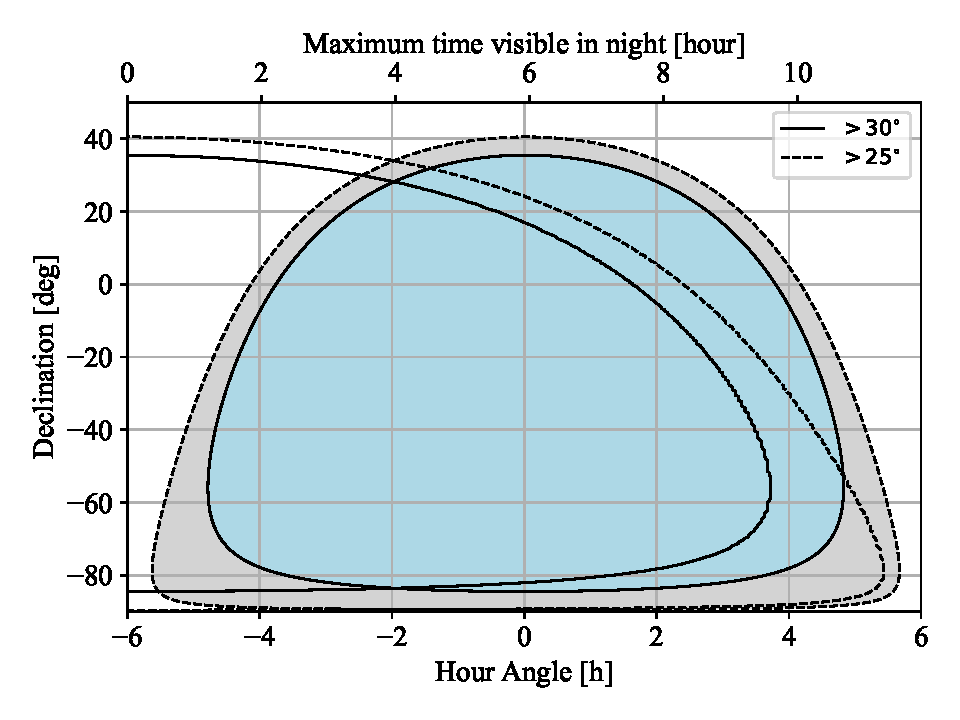
\includegraphics[width=\columnwidth]{NGTS_visibility.pdf}
    \caption{(upper panel) Contours marking the visibility from \ngts. Grey contours bounded by black-dashed lines marks the extent at which any given target can be observed above $25^{\circ}$. Blue contours bounded by solid black lines marks the extent at which any given target can be observed above $30^{\circ}$. The top axis shows the maximum time a target is visible above $25^{\circ}$ (black-dashed) and $30^{\circ}$ (black-solid).}
    \label{fig:ngts_visibility}
\end{figure}

\ngts\ is located alongside the VLT at the ESO Paranal Observatory in Chile, making it well suited to obtain precise photometry and support one of the best spectrographs in the world, \espresso \citep{2010SPIE.7735E..0FP}. Paranal is one of the best site in the world for our science, with an exceptional 78\% of photometric nights, and extremely dry conditions that minimises noise at red wavelengths due to water absorption. \ngts\ has good access to the Southern sky (Figure~\ref{fig:ngts_visibility}) and is capable of monitoring targets with declinations as far north as $+20^{\circ}$. Simultaneous observations between \ngts\ and \espresso\ provide exceptional complimentary science, and \ngts\ has also supported  campaigns to observe longer period planets which require longitudinal coverage of many observatories to monitor exceptionally wide transits. \ngts\ has vast synergies with the \tess\ mission and routinely observing TOIs, community TOIs, and candidates found from dedicated searches for long-period planets. Cerro Paranal is well-matched to observations in the Southern Ecliptic and provides some limited scientific support for targets in the Northern ecliptic. With the launch of \plato\ forthcoming, \ngts\ has unprecedented access to the Long-duration Observation phase Southern field 2 (LOPS2) field and can help with candidate validation, simultaneous observations, and pre-surveys. These cases are further discussed in Section~\ref{sec:related}.



\subsection{Precision}

\begin{figure*}
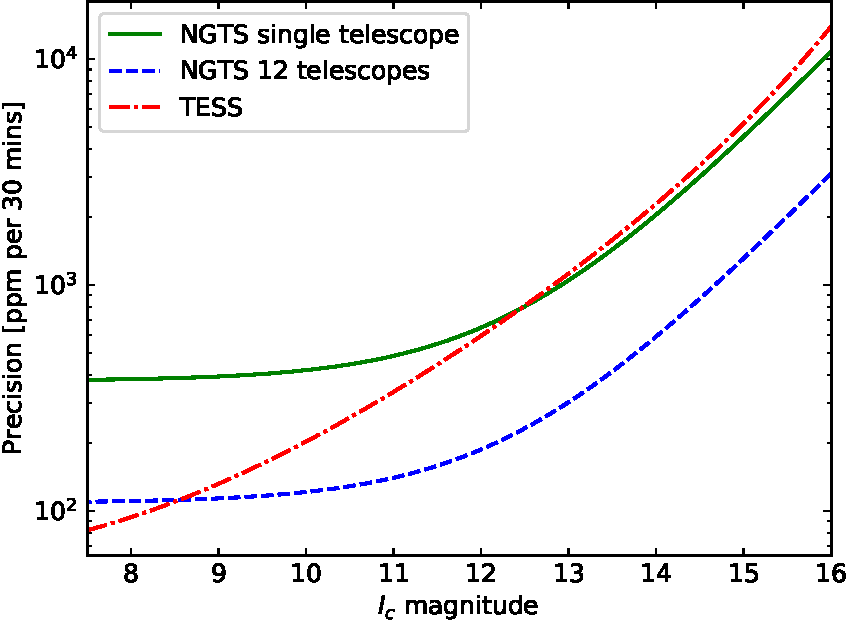
\includegraphics[width=7.0cm]{2508_ngts_tess_plot.pdf}
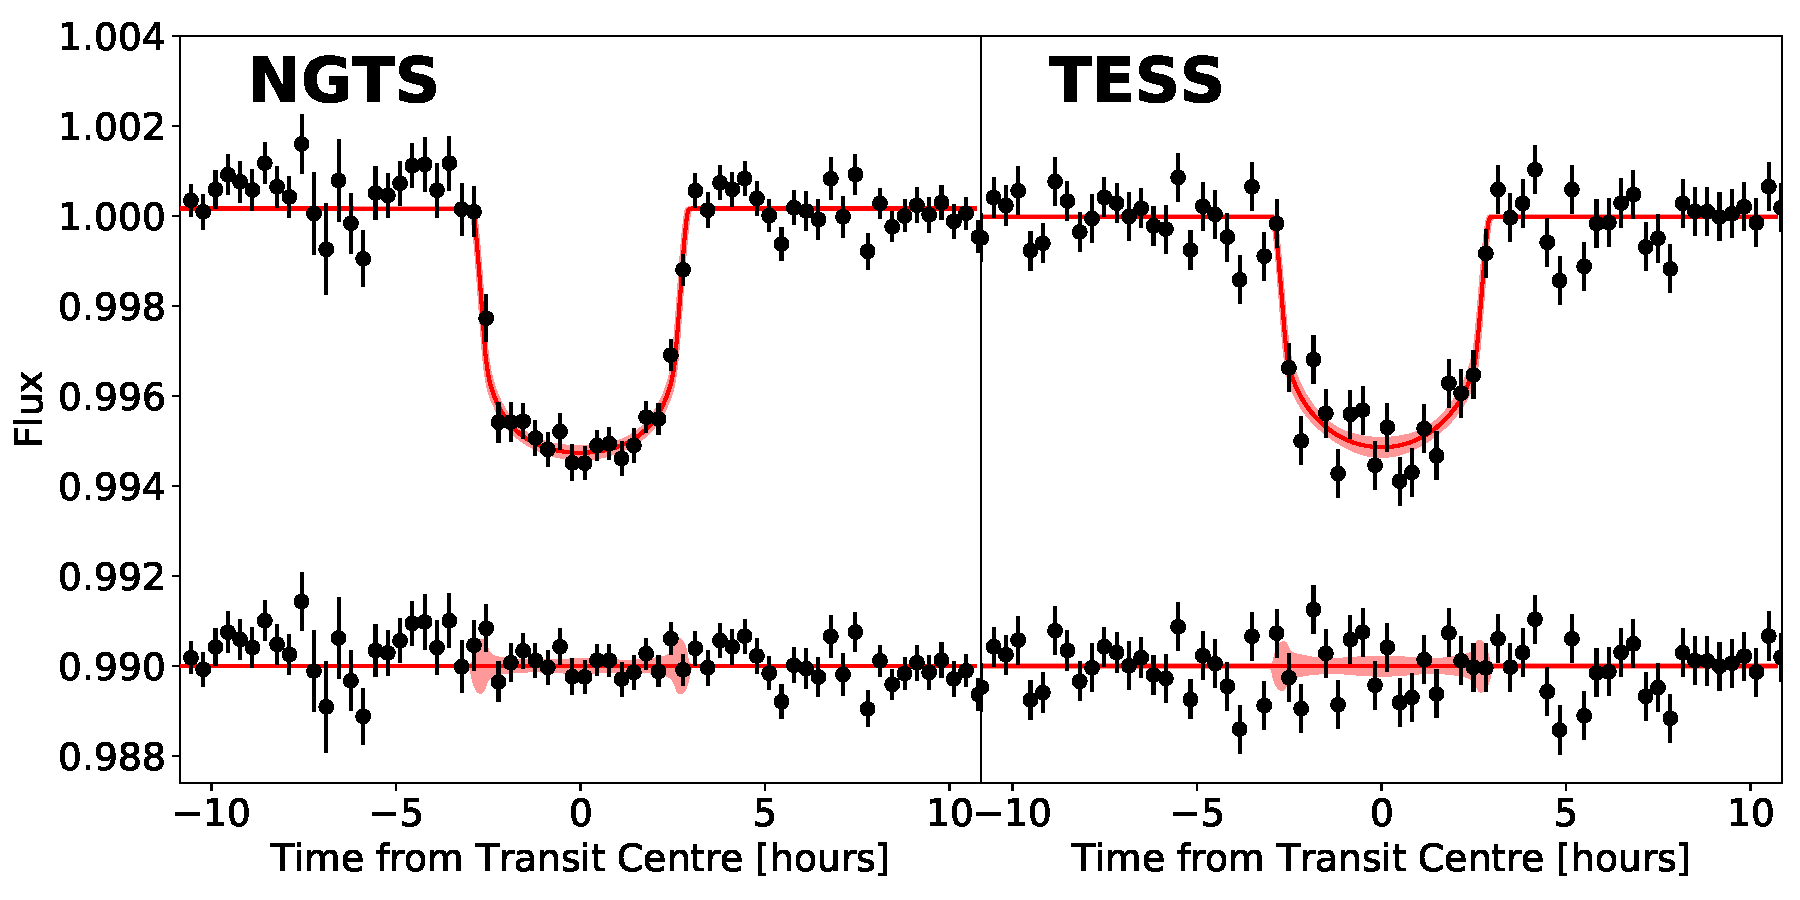
\includegraphics[width=10.4cm]{NGTS12_ngts_vs_tess_phase_fold_phot.pdf}
\caption{{\bf Left:} a comparison of photometric noise models for a single NGTS telescope (green solid line), 12 NGTS telescopes (blue dashed line), and \tess\ (red dot-dashed line). NGTS and \tess\ have similar photometric  precision for 12th magnitude and fainter. For brighter stars NGTS is limited to 400\,ppm by atmospheric scintillation.  However by using 12 telescopes simultaneously, NGTS can reach 100\,ppm, and produce higher photometric precision than \tess\ for stars right up to 9th magnitude (see Fig.\,\ref{fig:wasp166}). {\bf Right:} the phase-folded NGTS and \tess\ discovery light curves for NGTS-12 ($G$=12.1), with solid red lines giving best fit models \citep{bryant20b}. The NGTS light curve is from a single camera with a monitoring campaign of 660 hours (rms=400\,ppm).  The \tess\ light curve from Sector 10, which totals 510 hours of observing (rms=450\,ppm).  Due to the large \tess\ pixels, the target is partially blended in the \tess\ photometry, resulting in lower photometric precision and a slightly shallower transit depth. 
\label{fig:ngts_precision}}
\end{figure*}


\begin{figure}
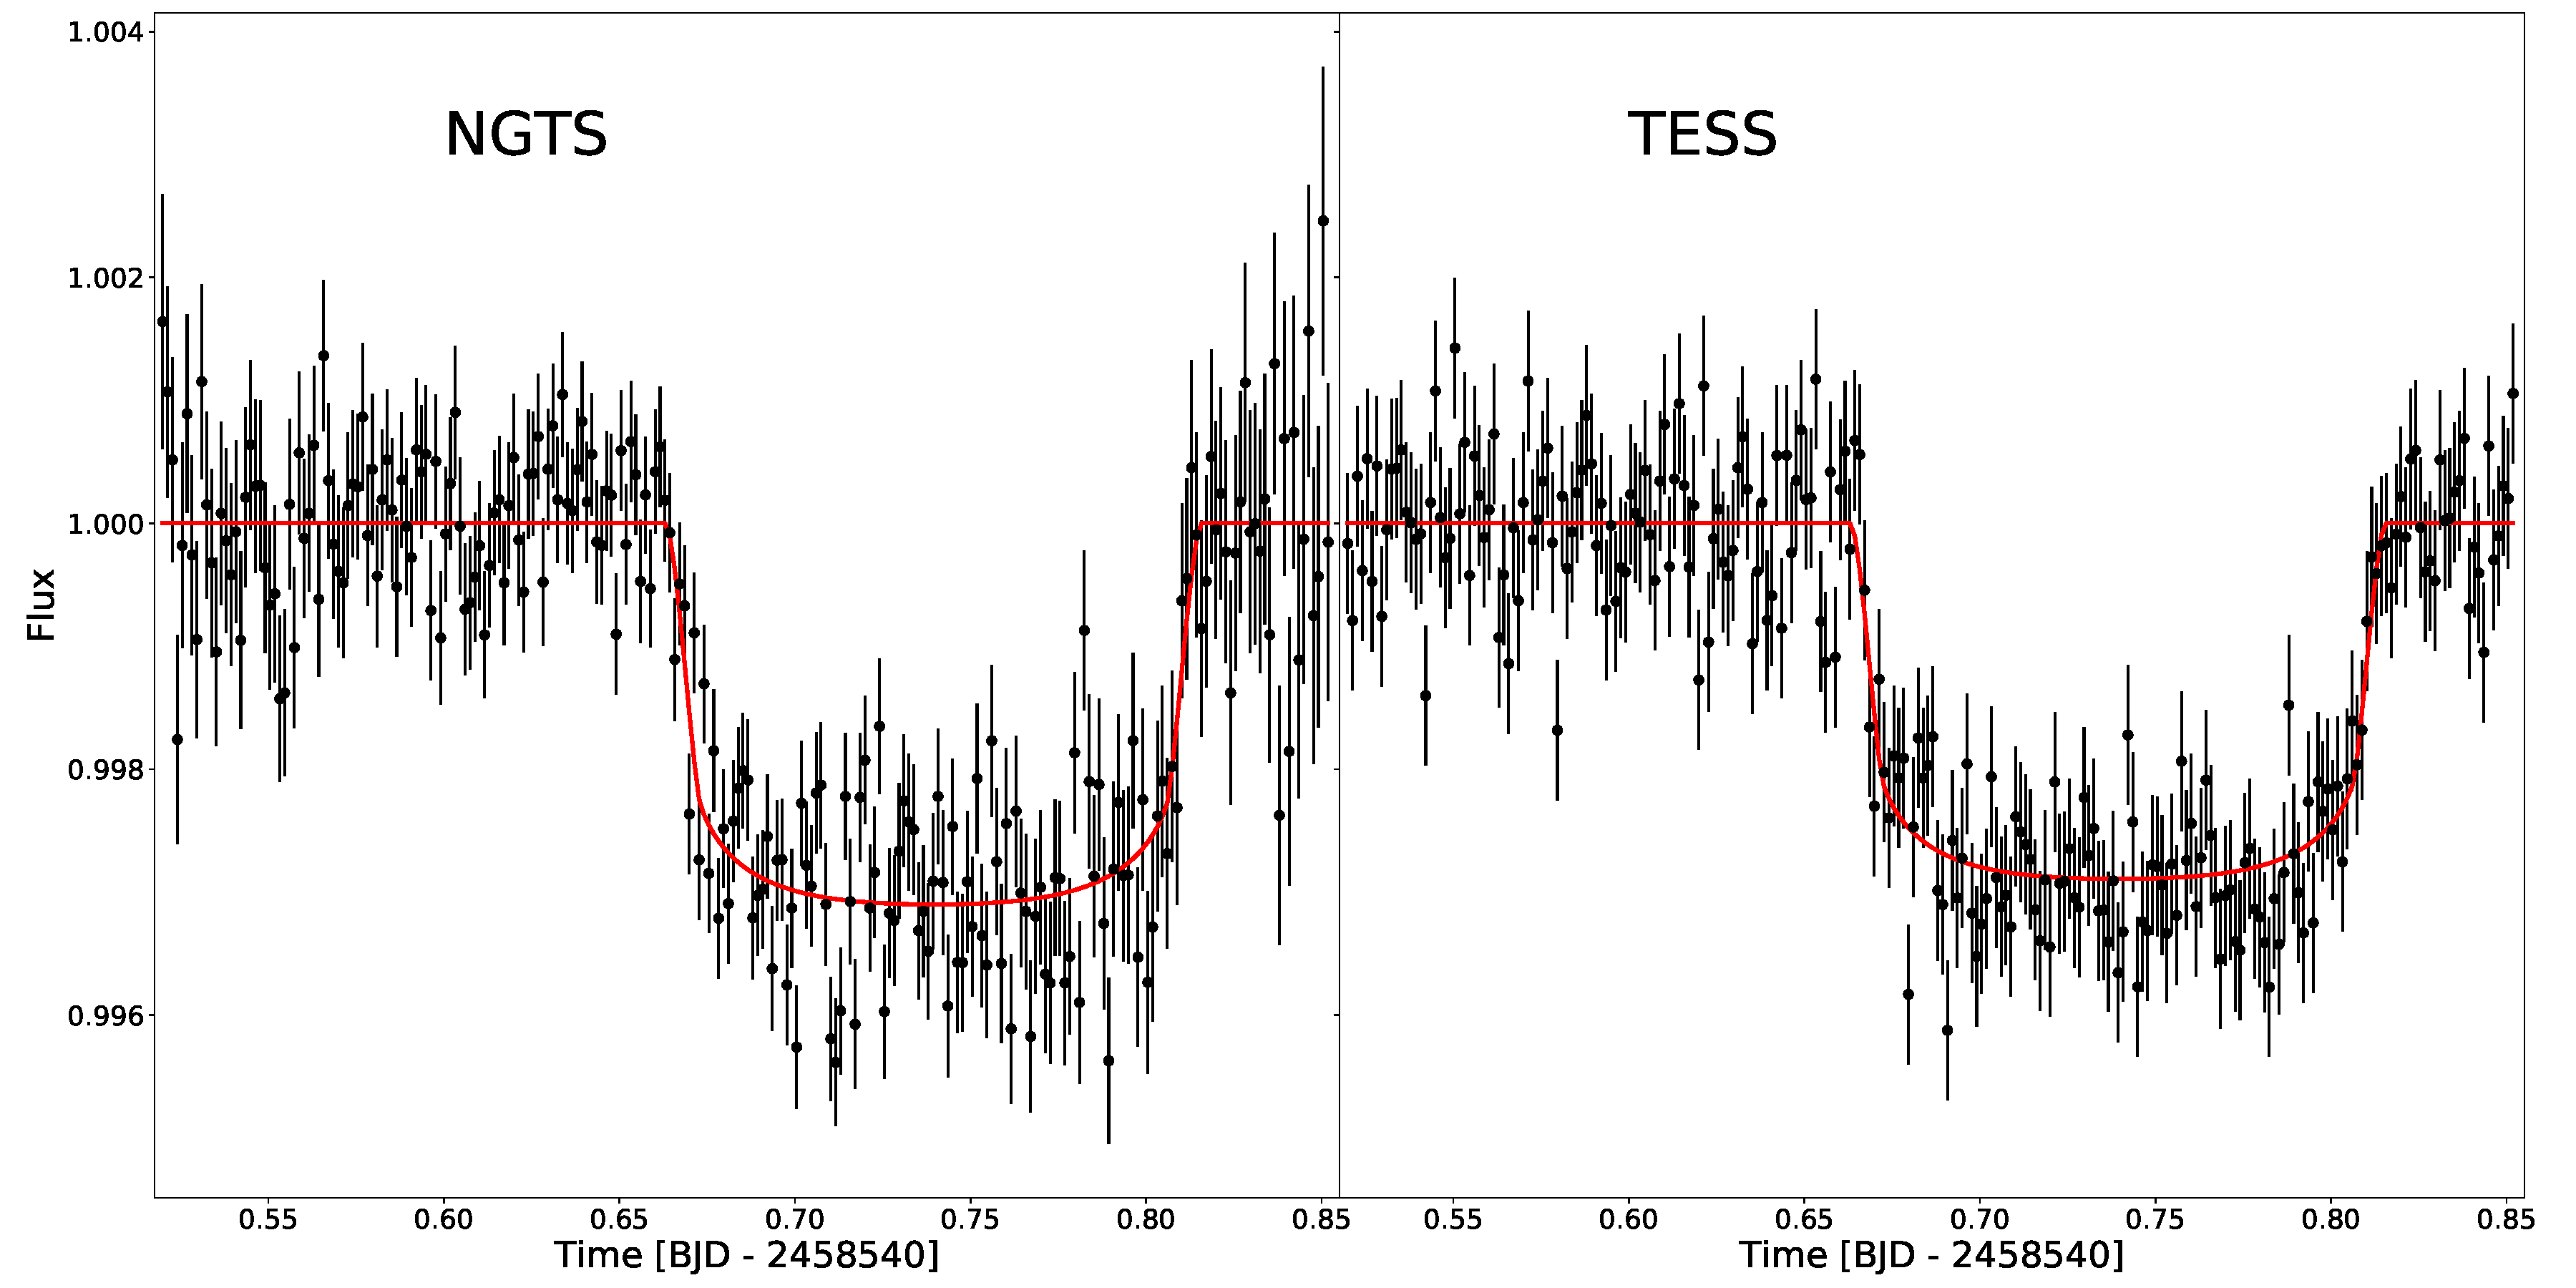
\includegraphics[width=\columnwidth]{WASP166_ngts_vs_tess_lcs.pdf}
\caption{A single transit of WASP-166\,b across its bright parent star ($G$=9.3) on 25 Feb 2019 as observed with \ngts\ (left) and \tess\ (right).  The \ngts\ light curve combines data from nine \ngts\ telescopes observing simultaneously. Data are binned to 2\,minutes, and the solid red line shows the best-fitting transit model. Plot from \citet{bryant20}.}
\label{fig:wasp166}
\end{figure}


\ngts\ is one of the most precise photometric facilities in operation.  To put this into context, in Figure\,\ref{fig:ngts_precision} we compare noise models for \ngts\ and the \tess\ mission. A single \ngts\ telescope is expected to have the same photometric precision as \tess\ for stars fainter than G=12, and in practice we usually out-perform \tess\ due to blending and scattered light (which are not accounted for in the \tess\ noise model). Brighter than G=12, a single \ngts\ telescope provides photometric precision of 400\,ppm (0.04\%) in 30\,min, which is limited by atmospheric scintillation. Since scintillation is white noise, and the NGTS data are essentially free of red noise, this precision continues to improve with binning. 

As an example of the precision we achieve with a single telescope, we present the discovery light curves of NGTS-12\,b in the right-hand panel of Fig.\,\ref{fig:ngts_precision} \citep[from][]{bryant20b}. NGTS-12\,b is a low-density 7.5\,d period transiting planet orbiting a G=12.1 host star. In total, the \ngts\ and \tess\ exposure times are similar (660\,h for \ngts, 510\,h for \tess) and yet a single \ngts\ telescope out performs \tess\ in this magnitude range. It is also worth noting that the \tess\ transit depth is slightly shallower than \ngts\ due to partial blending with neighbouring stars, which is a common problem with \tess\ photometry.  This blending also increases photometric noise in the \tess\ data.


%We can further reduce 
Brighter than G=12, we can overcome
scintillation noise by combining data from multiple \ngts\ telescopes observing simultaneously. The noise model in Fig.\,\ref{fig:ngts_precision} shows that by combining data from all twelve telescopes we can reach a precision of 100\,ppm in 30\,min. This approach is confirmed with real observations, and in Fig.\,\ref{fig:wasp166} we show a single transit of WASP-166\,b observed simultaneously with \tess\ and nine \ngts\ telescopes \citep{bryant20}. WASP-166 has a G magnitude of 9.3, and at this brightness it can be seen that nine \ngts\ telescopes have approximately the same precision as \tess. 

We note that in principle it is also possible to overcome scintillation noise by using an larger aperture telescope,  but for bright stars \ngts\ is able to take advantage of its wide field-of-view to ensure sufficient reference stars are monitored. This is usually not possible for the narrower fields of view of 1m-class telescopes. The individual \ngts\ telescopes, with 8\,deg$^2$ FoV, are in a unique position in providing sub-millimag relative photometry for the brightest \tess\ candidates right down to $G$$\sim$6.  By using all 12 \ngts\ telescopes simultaneously on a single bright target, we create a very wide field instrument with an effective collecting area of a 0.7m telescope and the scintillation noise of a 1.3\,m telescope \citep[scintillation is the limiting noise source for bright stars, see][]{2022MNRAS.509.6111O}.  In such a configuration, we can achieve 100\,ppm per 30 minutes for bright stars --- see Figs.\,\ref{fig:ngts_precision}\,\&\,\ref{fig:wasp166} and \citet{bryant20}.






% Next paragraph talk about WCS precision and how it does not rotate at the edge of fields

\begin{figure}
    \centering
    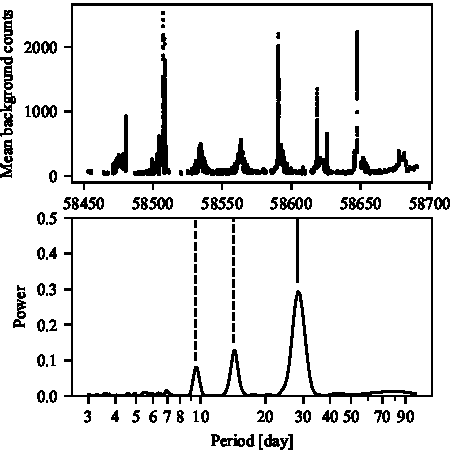
\includegraphics[width=\columnwidth]{IMAGE80120181201055814_moon.pdf}
    \caption{(upper panel) The mean background counts for a season of observations of a centred around RA = $10^{h}$ 19', Dec = $-33^{\circ}$ 35'. (lower panel) The Lomb-Scargle power spectrum for these observations. The black-solid line marks the variation caused by the lunar cycle while black-dashed lines mark its first two aliases.  }
    \label{fig:ngts_lunar_cycle}
\end{figure}

The optical and mechanical design along with the precise polar alignments of \ngts\ is optimised such that rotation of sources near of the edges of the CCD will move by less than 1 pixel across a given night. Baffles have been fitted to mitigate light contamination from the moon, however lunar cycles are still prominent in the background of \ngts\ images (Figure~\ref{fig:ngts_lunar_cycle}) which may be important for stellar activity monitoring observations. Fields that are observed through increasing airmasses are subject to an increased sky background contribution. For example, a field observed at airmass 2 can expect almost twice the sky background contribution compared to an observation at airmass 1, before additional contributions from scattered moonlight and high-altitude clouds. 




\subsection{Scheduling observations}

Each of the 12 telescopes is fully robotic and can observe between $\pm5.3$ hours in Hour Angle and between 
Declinations of +20 and -90$^{\circ}$. Telescopes are typically operated independently allowing the facility to multi-task 12 separate observing sequences. However, when increased precision is required, multiple telescopes can co-point at the same field and observations can be combined to improve the signal-to-noise ratio of the photometry. This is possible thanks to two features of NGTS. Each telescope autoguides using a long-term reference image (typically the first image of a field) and the \textsc{donuts} algorithm \citep{2013PASP..125..548M} to achieve exceptional sub-pixel stability over many nights of observations. This results in minimal correlated noise from each telescope. Additionally, the separation of each telescope is sufficient to break any correlation in atmospheric scintillation. As the telescope are essentially free from correlated noise and the scintillation noise between adjacent telescopes is uncorrelated, we can combine data from multiple exposures within a telescope and data from multiple telescopes to achieve exceptional photometric precision ({\color{red} get some numbers and reference one of the previous papers}).

A typical night per telescope consists of evening flats, a focus sweep, a number of scientific observing blocks, morning flats and bias/dark exposures after the roof has closed. Each of these phases is defined by an NGTS action. Each action type requires a distinct set of parameters, this typically includes values for the action type, start time, end time and any action specific parameters, such as target count levels for flats or the span of a focus sweep. This information is entered into a MySQL database table by the NGTS scheduler. Each telescope's control system (\textsc{paladin}) subsequently fetches jobs in real time to execute the night's sequence. All actions are scheduled based on Sun elevation (e.g. roof opens at Sun elevation of 1.0$^{\circ}$, dusk flats start at -4.5$^{\circ}$ and science observations begin at -15$^{\circ}$.)

The NGTS scheduler divides all science observations into one of two observing modes, time critical or survey. Time critical mode captures any observations where the user specifies the start and end time of the observations. Survey mode is less strictly defined and a target is essentially valid the entire time it meets the observability constraints of the telescope (e.g. sufficiently high above the horizon and far from the moon etc). Start and end times of survey observations are then defined by overlapping target priorities and observabilities. Assigning priorities to each target is usually where the complexity in any scheduler lies. We completely avoid managing priorities within the NGTS scheduler logic. The priority complexity is offloaded to the NGTS working group users. Working groups divide the total observing time amongst themselves and agree on the relative priorities of the different active projects running on NGTS.

The scheduling logic is therefore extremely simple, it must guarantee that the highest priority target at any given time on a given telescope is attempted.  Through collaboration, the different working groups assign a priority to each target on an integer scale between 0 and 10, where 0 is the highest and 10 is the lowest priority. Priorities are assigned using odd numbers only and 0 priority is reserved for the most important targets and is rarely used. Using odd number priorities gives the flexibility of injecting targets at short notice between existing scheduled observations. This is achieved by inserting new requests with the corresponding even numbered priority level to trump (or not) existing requests. By definition time critical observations are given higher priorities than survey type observations. 

The observing night for each telescope is defined as the window when the Sun is below -15$^{\circ}$ elevation. This window is broken up into 1 minute steps and the scheduler calculates the highest priority target for each step. The scheduler combines each target's priority with its airmass to give a measurement of \emph{importance}. The importance of all targets is evaluated across all 1 minute time steps in an initial pass. A second pass over each telescope's schedule then determines the start and end time of continuous observing blocks of the targets with the highest importance (priority). Scaling the priority by airmass automatically allows for survey targets with equal priority to hand over at the optimal airmass. This minimises the amount of time spent observing at high airmass. 

The nightly schedule for each telescope is made ahead of time compromising of observations in time critical mode and lower priority survey fields. Best efforts are made to use the same cameras when observing targets for more than one night to avoid systematic offsets from the different photometric zero-points of each camera.

Default values for elevation limit, moon avoidance angle and time spent observing in twilight etc are preconfigured, but the scheduler allows these to be overridden by some safe margin should the need exist. The scheduler has an additional set of safety limits for such parameters beyond which the system will never be pushed.

At the end of the night, images are compressed with the \textsc{bzip2} algorithm \citep{seward_bzip2} and moved to a centralised storage at Cerro Paranal. Synchronisation with centralised storage at the University of Warwick may take up to a few months as data is transfered back in bulk on removable 6TB hard discs. 


\subsection{Complementary projects}\label{sec:related}

The capabilities of \ngts\ complement other leading observatories and telescopes. In this section we detail a few cases where \ngts\ has complemented studies of exoplanets and beyond. 


\subsubsection{TESS}
\label{sec:tess}

The Transiting Exoplanet Survey Satellite (\tess; \citealt{Ricker15}) is a NASA explorer-class spacecraft carrying out a wide-field search for transiting exoplanets around bright stars.  \tess\ began science operations in July 2018, and in its primary mission (the first two years of operation) it surveyed approximately 80\% of the sky.  \tess\ is now carrying out an extended mission where it re-surveys large areas of the sky.  As of 1 August 2021 there are \textbf{4404 \tess\ exoplanet candidates and 144 \tess\ confirmed planets (\url{https://exoplanetarchive.ipac.caltech.edu})}. The primary science goal is to measure the masses of 50 transiting exoplanets with $R_P<4R_{Earth}$.  

With the benefits of a space environment (stability, no atmospheric scintillation, no diurnal cycle), \tess\ has become the pre-eminent survey for discovering transiting exoplanet candidates.  However there are some critical limitations.  \tess\ surveys fields with 27-day sectors, so it finds short period transiting exoplanets with ease (P$<$10\,d), but largely misses the longer period (cooler) planets. Exoplanet which transit once or twice in \tess\ may require extensive follow-up to determine the true orbital period. \ngts\ is one of the only facilities in the world capable of efficiently solving the orbital period of long-period planets from \tess\ and has become one of the main science objectives of \ngts\ \citep{2020MNRAS.491.1548G,2020ApJ...898L..11G,2022MNRAS.513.1785G,2024MNRAS.532.1444G}. Additionally the large pixels of \tess\ (21\,arcsec) means that photometric blending of sources is a serious issue for many stars \citep{2015ApJ...809...77S}. 

\ngts\ is able to complement \tess\ to overcome these issues. The \ngts\ pixel scale is much finer (5\,arcsec/pixel), and therefore many blended sources are resolved. Finally, \ngts\ provides some of the highest cadence photometry of any transit survey (13\,s), allowing for transit shapes to be accurately mapped (c.f. \tess\ full-frames images are currently at 10 minute cadence).  This is particularly relevant for short duration events, such as transits and eclipses of white dwarfs \citep[e.g.][]{2021MNRAS.502..581C}.  It is also important to note that the noise properties of a single \ngts\ telescope and \tess\ are identical for objects fainter than $G$=12 magnitude (including most M dwarfs, white dwarfs and main sequence stars in open clusters). The \ngts\ project works closely with the \tess\ mission, with \ngts\ members heavily involved in the \tess\ Follow-Up Program (TFOP). In particular, \ngts\ members are active in TFOP Sub-Group 1 (Photometric Follow-up) and TFOP Sub-Group 4 (Radial Velocity Follow-up).  

However, there is a serious problem with photometric follow-up of these candidates from the ground.  This is because reference stars of similar magnitude to the target need to be monitored within the field-of-view (FoV) of the instrument in order to produce high-precision relative photometry. On average, for $G$$<$10 candidates, this requires a FoV larger than 0.5\,deg$^2$. Although the TFOP Sub-Group 1 has assembled a large team for photometric follow-up of \tess\ candidates, the typical FoV of the instruments in this group is 0.09\,deg$^2$, and none are larger than 0.44\,deg$^2$ \citep[see FoVs listed in Table 2 of][]{2018AAS...23143908C}. Thus in most cases, none of these telescopes can achieve high precision on $G$$<$10 \tess\ candidates.

Over the past three years we have used \ngts\ in this multi-telescope mode to provide sub-millimag photometry for bright TOIs \citep{2020Natur.583...39A,2019ESS.....410307J,2020A&A...639A..76N,2021MNRAS.507.2782O,2022MNRAS.510.5464K,2023MNRAS.520.3649H}. We plan to continue to follow-up  new bright TOIs that will emerge from the \tess\ extended mission.  In addition, we are carrying out extended (multi-year) monitoring campaigns of bright transiting planet systems that show transit variability - either due to to dynamical interactions in multi-planet systems or star-planet interactions for ultra-short period systems.  We have already successfully measured a large transiting timing variation for the 542\,d-period ultra-low-density HIP\,41378\,f \citep{2021MNRAS.504L..45B}, as well as transit timing variations in the TOI-270 system \citep{2019NatAs...3.1099G}. 











\subsubsection{CHEOPS}
\label{sec:cheops}
\cheops\ \citep[CHaracterising ExOPlanet Satellite;][]{2021ExA....51..109B} is an ESA S-class mission that was launched in December 2019. It consists of a 0.3-m telescope designed to perform high-precision photometry for precise measurements of planetary radii. \cheops\ differs from \tess\ in that it is a dedicated follow-up mission, rather than a survey instrument. It observes a single star at a time, with a heavily defocused image mapped on to a frame-transfer CCD -- enabling high-cadence, high-precision photometry.

The synergy between \ngts\ and \cheops\ is a result of the differing capabilities of the two observatories, coupled with several shared science goals. \ngts\ is much better suited to long-term monitoring of a target (such as that needed to eliminate period aliases from a \tess\ single-transit event), while the superior photometric precision of \cheops\ enables the measurement of shallower transits, and higher-precision radius determination than is possible from the ground.  The twelve telescopes of \ngts\ can be split between several targets, allowing for monitoring of many more transiting candidates.  By contrast, \cheops\ uses its limited time to observe a smaller number of candidates - generally those that are too shallow to detect reliably from the ground.  \ngts\ can also observe objects at southern declinations which are out of reach for \cheops.

The harmony between \ngts\ and \cheops\ is demonstrated by the study of the six planet TOI-178 system \citep{2021A&A...649A..26L}.  \tess\ initially identified three planet candidates around the star, with periods of 6.55, 10.35, and 9.96\,d \citep{2019A&A...624A..46L}. Targeted \ngts\ observations revealed only one of two predicted transits of the 10.35-d planet. These observations, together with \cheops\ observations, enabled us to determine that the apparent 10.35~d signal was actually caused by a planet orbiting with a 20.7\,d period, with one of the 10.35-d transits observed by \tess\ attributed to an additional planet at 15.2\,d. \cheops\ observations also confirmed two inner planets at 1.9 and 3.2\,d. Together the outer five planets form a remarkable 2:4:6:9:12 chain of Laplace resonances, and TOI-178 is now a benchmark multiple planetary system.



\subsubsection{ESPRESSO}

\espresso\ (Echelle Spectrograph for Rocky Exoplanets and Stable Spectroscopic Observations; \citealt{2010SPIE.7735E..0FP}) is an ultra-stabilised spectrograph on ESO's 8m VLT telescopes at Paranal Observatory.  It is designed to measure radial velocities at a precision high enough to detect true Earth-like planets (10\,cm\,s$^{-1}$), making it the most precise radial velocity instrument in operation.  In addition to its high precision, \espresso\ can be fed with up to four of the 8m VLT telescopes, meaning it can monitor much fainter stars than is possible with existing facilities such as HARPS \citep{2002Msngr.110....9P}.  This opens the way for radial velocity monitoring of many optically faint, but scientifically interesting, targets such as M-dwarfs. 

\espresso\ will be used to measure the masses and characterise the atmospheres of many small exoplanets detected by \tess\ and validated with \ngts. Given the time pressure on the VLT, validation of \tess\ candidates is critical in order to remove false positives from blended eclipsing binaries. \ngts\ will also support \espresso\ observations by taking simultaneous high-precision photometry that allows systematics from stellar activity to be detrended. This is particularly valuable for transit observations, where star-spot crossings and unocculted spots can contaminate Rossiter-McLaughlin measurements and transmission spectroscopy. Since the two instruments are co-located, \ngts\ is always available when \espresso\ is taking data and has provided numerous simultaneous observations \citep{2022MNRAS.516..298D,2023MNRAS.522.4499D}. 

\subsubsection{PLATO}

\plato\ is an ESA M-class mission due for launch in 2026. It is designed to characterise stars using asteroseismology and to find transiting exoplanets as small as the Earth around bright Sun-like stars, including in the habitable zone \citep{2014ExA....38..249R}. 

\plato\ differs from \tess\ in that it builds signal-to-noise by employing multiple small telescopes with overlapping fields of view. This is similar to how \ngts\ obtains precise photometry of transiting exoplanets and some synergies are becoming apparent. These can include a pre-survey of the \plato\ fields, follow-up of intermediate-sized transiting planets once \plato\ has moved on to a new field including period confirmation and TTV monitoring, eclipsing white dwarfs, long-period variable stars and benchmark eclipsing binary stars. 





\section{Image processing}\label{sec:preprocessing}

\begin{figure}
    \centering
    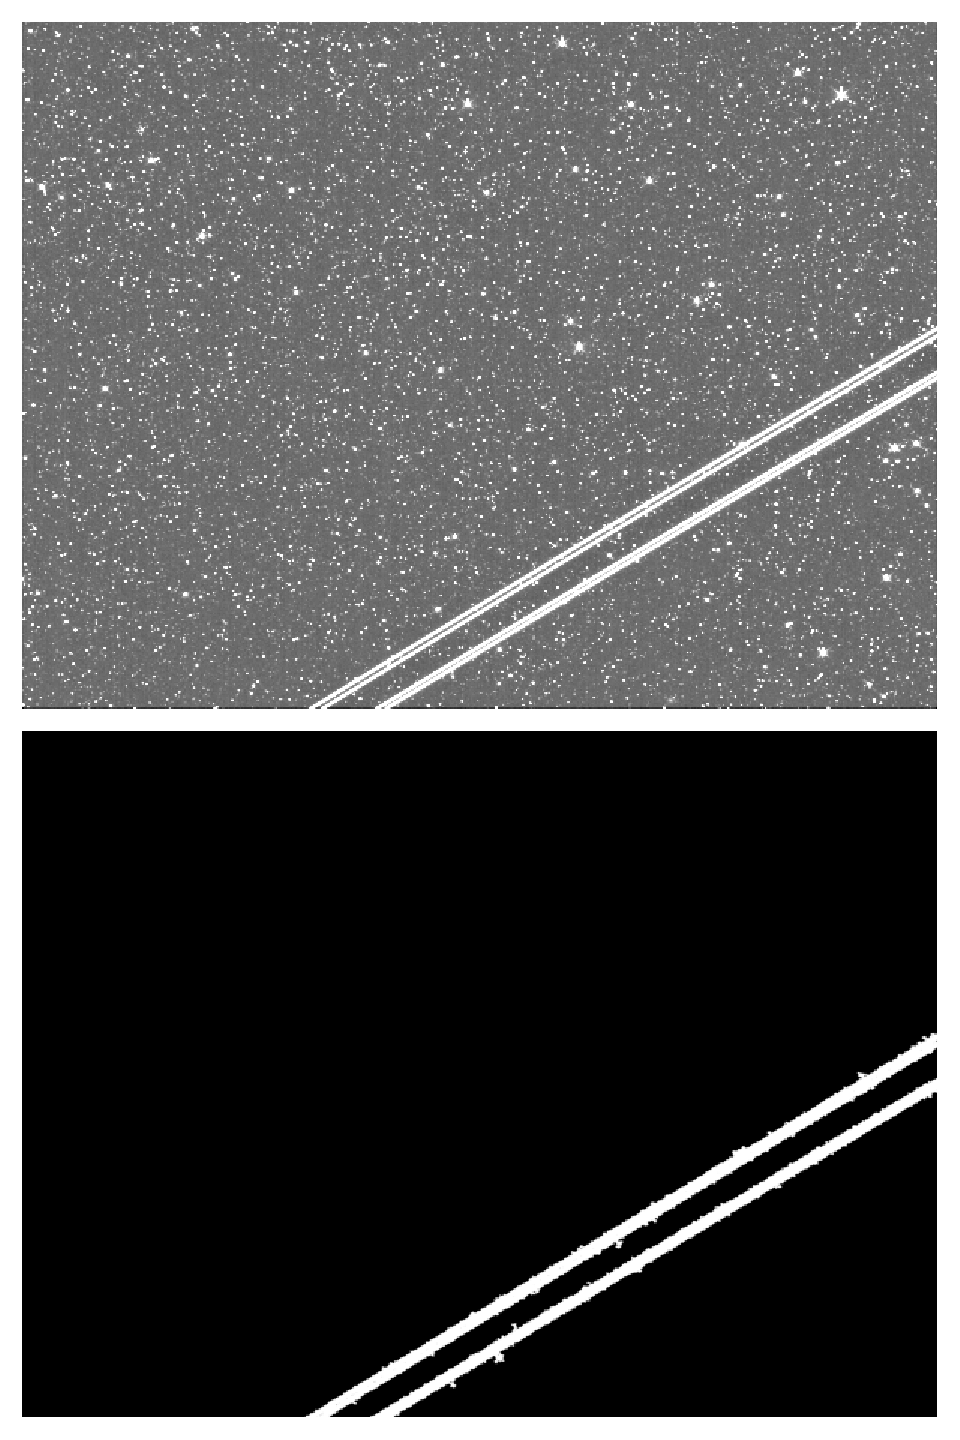
\includegraphics[width=\columnwidth]{Figure_3.pdf}
    \caption{(upper panel) Raw image of field centred around RA = $14^{h}$ 16', Dec = $-30^{\circ}$ 56' with the VLT laser clearly visible in the bottom-right corner. (lower panel) binary mask produced by our algorithm which identifies pixels affected by the VLT laser.}
    \label{fig:Figure_3}
\end{figure}

\begin{figure}
    \centering
    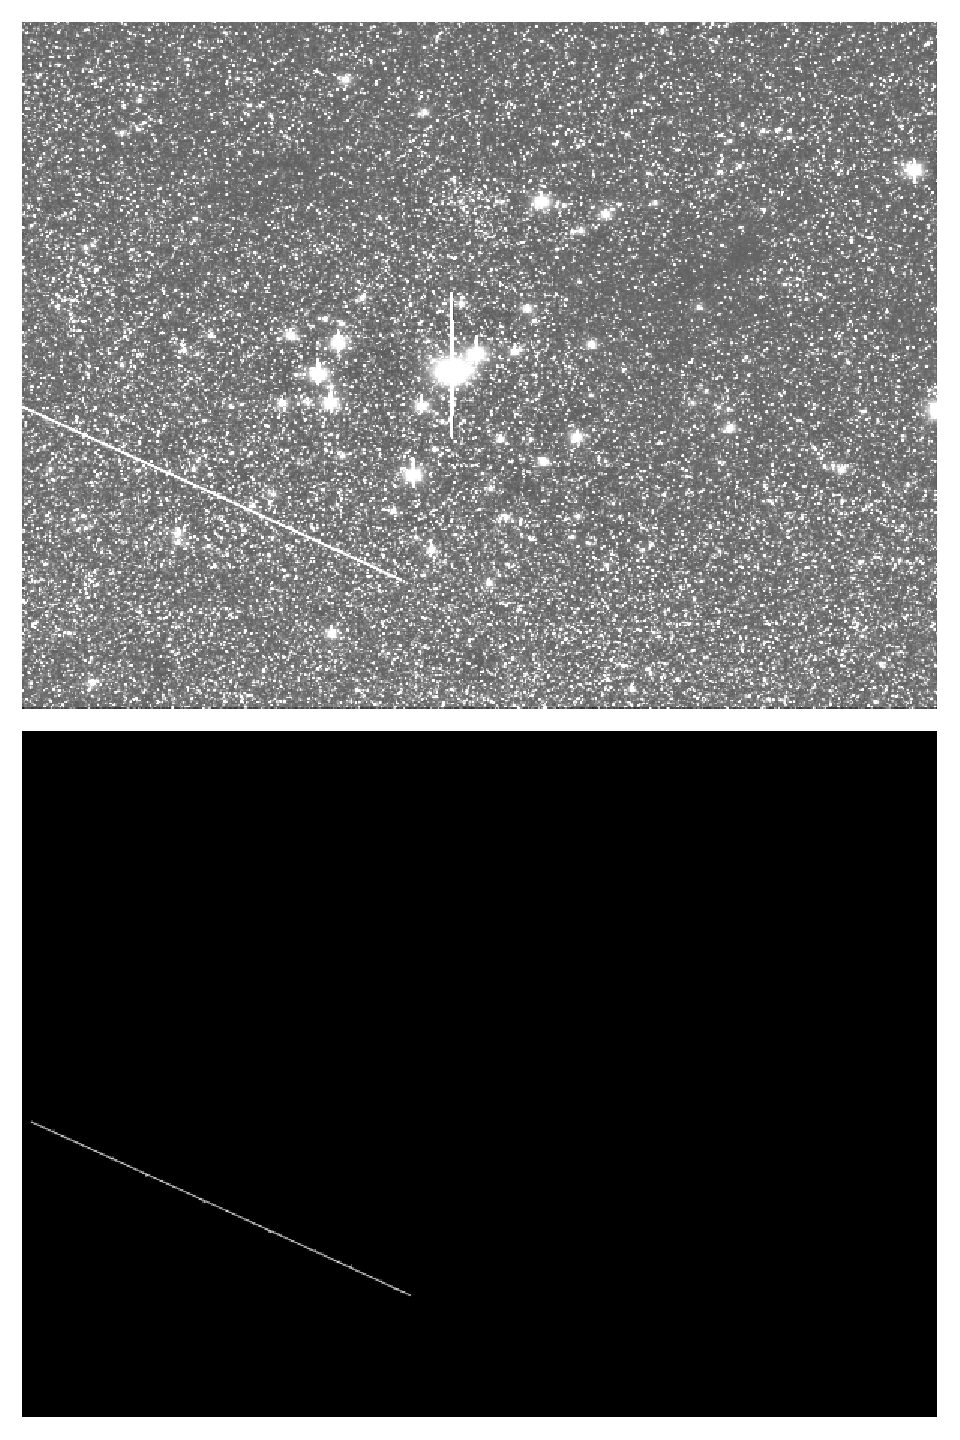
\includegraphics[width=\columnwidth]{Figure_3_sat.pdf}
    \caption{(upper panel) Raw image of field centred around RA = $10^{h}$ 42', Dec = $-64^{\circ}$ 25' (IC 2602) with a prominent satellite streak visible. (lower panel) binary mask produced \textsc{astride} which identifies pixels affected satellites.}
    \label{fig:Figure_3}
\end{figure}




The deep-depletion CCDs on NGTS have a 2048$\times$2048 illuminated pixel area. They also include unilluminated pre- and over-scan regions (the first and last 20 columns), yielding a raw image size of 2048$\times$2088 pixels. These regions are useful to determine small variations in the frame-to-frame bias level. Each image is cropped to remove the pre-/over- scan regions and the median count value in the over-scan region subtracted on a row by row basis. The over-scan corrected images are then used as our reduced science images.  We do not perform flat-field correction, remove dark current or perform further bias corrections similar to the main \ngts\ pipeline \citep[see][]{2018MNRAS.475.4476W}. We find the additional corrections yield no improvement on the photometric quality and are therefore not required to create publication grade lightcurves.  


\subsection{Laser detection}\label{sec:laser_detection}

The European Southern Observatory Very Large Telescope (VLT) comprises of four 8-m telescopes adjacent to \ngts\ at Cerro Paranal and hosts the 4 Laser Guide Star Facility \citep{2014AdOT....3..345C}. This system projects four laser beams into the atmosphere, exciting sodium atoms to create artificial stars that can be used to correct for atmospheric turbulence at each telescope's focal plane. Occasionally, these lasers traverse the field of view of \ngts\ telescopes. This will occur more often with plans for similar laser systems for the other three 8-m telescopes and the European Southern Observatory Extremely Large Telescope \citep[ELT;][]{2016SPIE.9908E..1XT}.

There exists a need to identify which \ngts\ images contain the laser and which pixels of those are affected. We first flag all pixels which exceed count values of 1000 adu and use a recursive algorithm to additionally flag other pixels nearby which exceed the median count value of the image plus $1$-$\sigma$. Pixels adjacent to each other are grouped together and the group is checked to see if it occupies two edges of the frame. If two edges are occupied by a group, we assume it is caused by the laser and flag all sources within 50 pixels of the grouped pixels. This algorithm, shown in Figure~\ref{fig:Figure_3}, effectively distinguishes laser artefacts from bright stellar sources. This is crucial for autoguiding with the \textsc{donuts} algorithm and flags photometric datapoints affected by the laser. 


\subsection{Satellites}

Satellites pose a significant challenge in astronomical image analysis due to their varied appearances, which can range from star-like points with slow motion across frames to long streaks, influenced by factors such as orbit, shape, size, and orientation relative to the Sun. The identification of slow-moving satellites within this pipeline is not pursued due to the difficulty in isolating them within individual images. Addressing this task would require a more intricate approach involving a sophisticated differential imaging routines capable of discerning anomalous sources that manifest as point-like entities across successive frames, a task that exceeds the current scope of this pipeline. For rapidly moving satellites we leverage the \textsc{astride} package \citep{2016ascl.soft05009K} specifically developed for detecting streaks in astronomical images through contour tracing. Originally devised for identifying swift-moving sources like meteors, satellites, or near-Earth objects, \textsc{astride} proves effective in detecting moderate-to-fast moving satellites. All pixels within 50 pixels of those affected by satellites are flagged; an example is shown in Figure \ref{fig:Figure_3}. This algorithm often incorrectly attributes pixels being within satellite streak, particularly around bright sources, and so this flag is used with caution.



\subsection{Estimating the sky background}\label{sec:backrgound}

\begin{figure*}
    \centering
    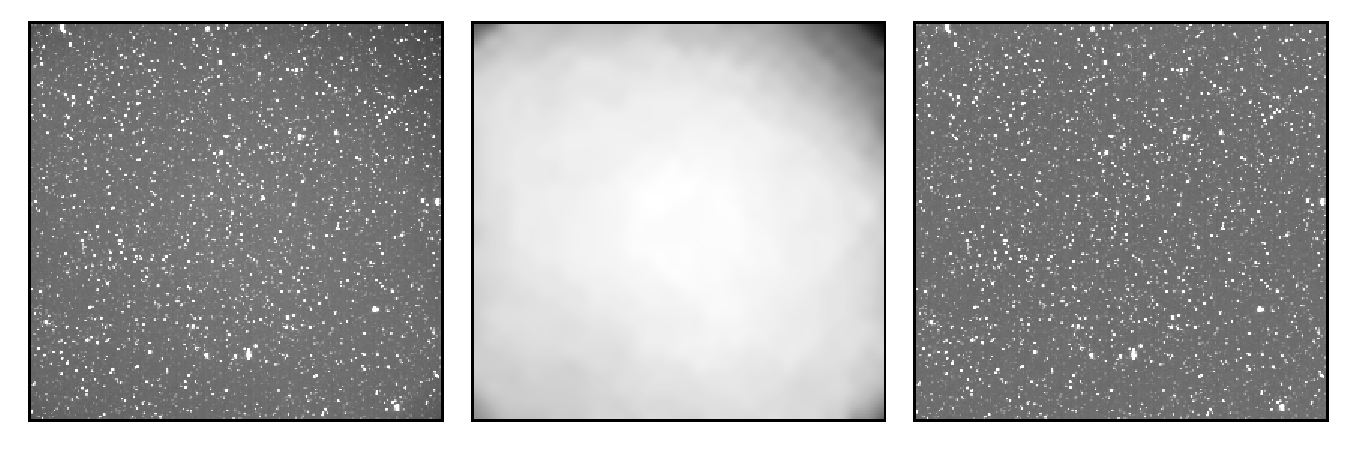
\includegraphics[width=\textwidth]{Figure_1.pdf}
    \caption{(left) Raw image of field centred around RA = $21^{h}$ 41', Dec = $-36^{\circ}$ 33'. (centre) The sky-back ground estimated for the raw image using \textsc{sep}. (right) The background-subtracted data used for aperture photometry.  }
    \label{fig:Figure1}
\end{figure*}

\ngts\ images feature feature non-uniform trends in the sky-background like many ground based observatories. These largely relate to optical design (e.g. vignetting and dust in the optical path) or atmospheric effects (e.g. Zodiacal light and Rayleigh scattering from Nitrogen, Oxygen, and aerosols). These effects decrease the contrast of the observed field such that an increase in photometric measurement error may observed inhomogeneously across the image. Photometric measurements and associated errors in \ngts\ images require spatial variable background maps. 

Iterative sigma clipping is used to identify pixel values exceeding $7$-$\sigma$ of the median value, often indicative of cosmic rays, satellites, or the adaptive optics lasers from the VLT (Section~\ref{sec:laser_detection}). A spatially variable background map is then generated utilising the \textsc{sep} package \citep{1996A&AS..117..393B,Barbary2016}. Parameters include a background box width and height of 128 pixels and a filter width and height of 3 pixels, broadly aligned with the full-width half maximum of the point-spread function in typical focused \ngts\ images. This background map enables the estimation and subtraction of sky-background flux contributions and yields a background-subtracted science image (see Figure~\ref{fig:Figure1}).



\subsection{Source detection}\label{sec:source_detection}


\begin{figure}
    \centering
    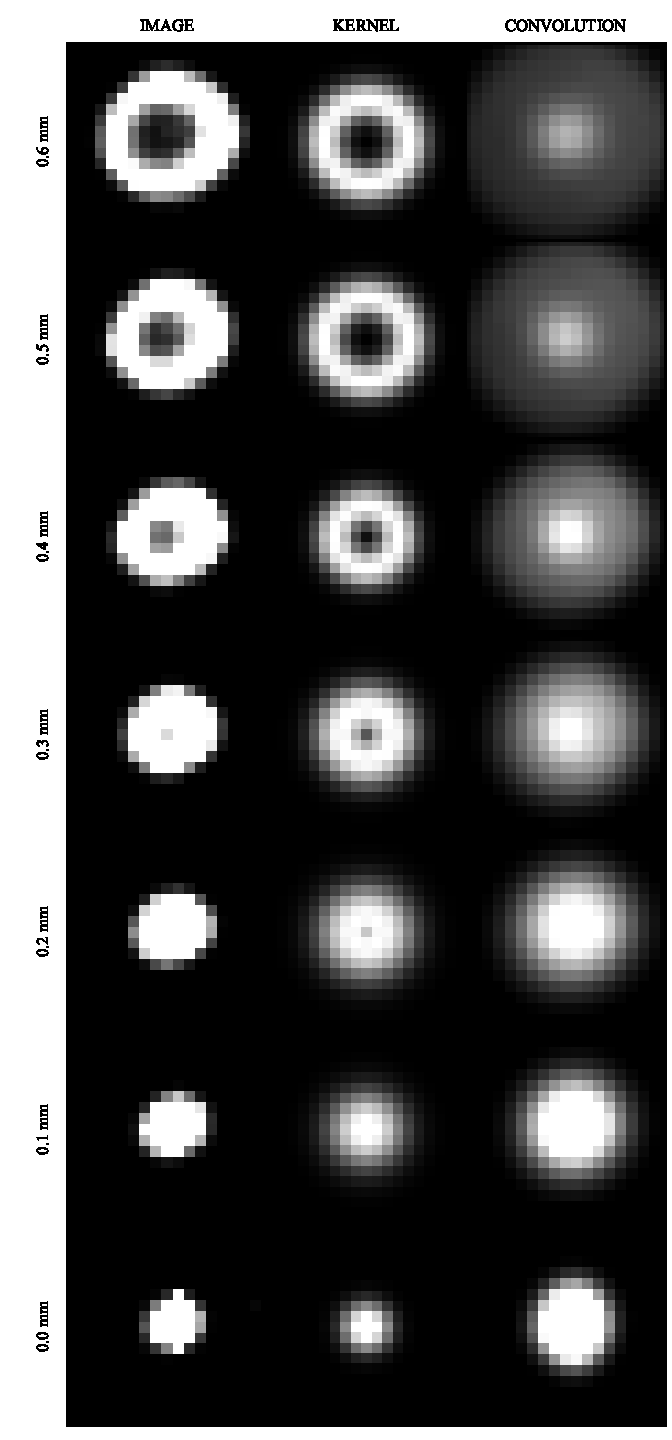
\includegraphics[width=\columnwidth]{kernels.pdf}
    \caption{Point spread functions of sources in \ngts\ images for various defocuses offsets [mm]. We also show the constructed kernel used for source detection in \ngts\ images, along with a convolution of the Point spread functions and the kernel. }
    \label{fig:detection_kernels}
\end{figure}

There is a need to accurately measure the exact positions of star such that the background can be robustly measured and to create the astrometric solution for the image. We use the \textsc{sep} function \textsc{extract} \citep{Barbary2016} which is built upon the framework of \textsc{sextractor} \citep{1996A&AS..117..393B}. A filtering kernel is required to ensure sources are robustly detected in defocused images as the point-spread function deviates from a Gaussian profile (of full-width half maximum of $\sim2$ pixels) to a broad donut shape. This is much larger than, and therefore independent of the astronomical seeing from Cerro Paranal. We imaged a quiet patch of sky with defocuses spanning 0\,mm (in-focus) to 0.6\,mm (maximum defocus) and measured the mean point-spread function of suitable stars in the field (left column of Figure~\ref{fig:detection_kernels}). For defocuses below 0.2\,mm, we fit Gaussian shape to each defocus level (0\,mm and 0.1\,mm) to establish the best filtering kernel (middle column of Figure~\ref{fig:detection_kernels}) . For defocuses equal and above 0.2\,mm, we fit a donut shape with inner radius and full-width half maximum of the outer ring to establish the best filtering kernel. Images with arbritrary defocus values use filtering kernels interpolated from these filtering kernels and allows for precise star positions to be measured from a matched-filtered image (right column of Figure~\ref{fig:detection_kernels}). 

This process yields a comprehensive list of source positions, their associated flux, and estimates of point-spread function shape parameters (ellipse parameters) for each \ngts\ image. This is used to determine a binary mask of pixels that contain flux from stars such that the sky background (Section~\ref{sec:backrgound}) can be reliable determined and enables the refinement of the world coordinate system (Section~\ref{sec:WCS_solution}).









\subsection{Determining the World Coordinate System}\label{sec:WCS_solution}

\begin{figure*}
    \centering
    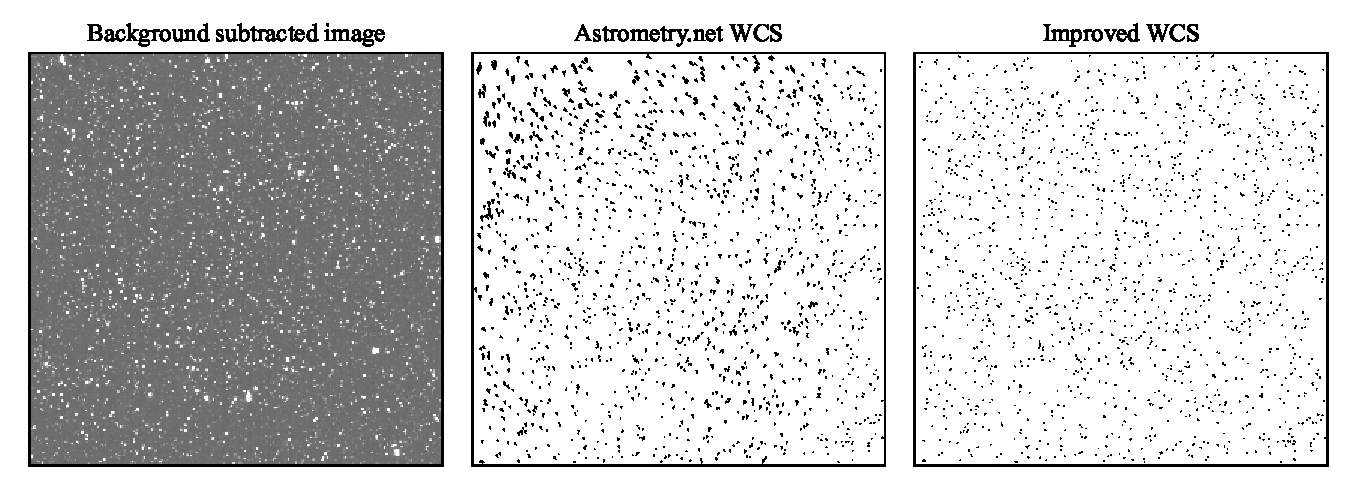
\includegraphics[width=\textwidth]{Figure_2.pdf}
    \caption{(left) Raw image of field centred around RA = $21^{h}$ 41', Dec = $-36^{\circ}$ 33'. (centre) A quiver plot for the astrometric solution of the left image found by Astrometry.net for suitably bright and non-blended sources. (right) The same for the improved WCS described in section \ref{sec:WCS_solution}. In both quiver plots we show only stars with maximum difference of 0.1 pixels between their measured position and their predicted position from the improved WCS to highlight the improvement. Each quiver is exaggerated by a factor of 100. A histogram of differences for the full sample is shown in Figure\,\ref{fig:Figure_4}.}
    \label{fig:Figure2}
\end{figure*}

\begin{figure}
    \centering
    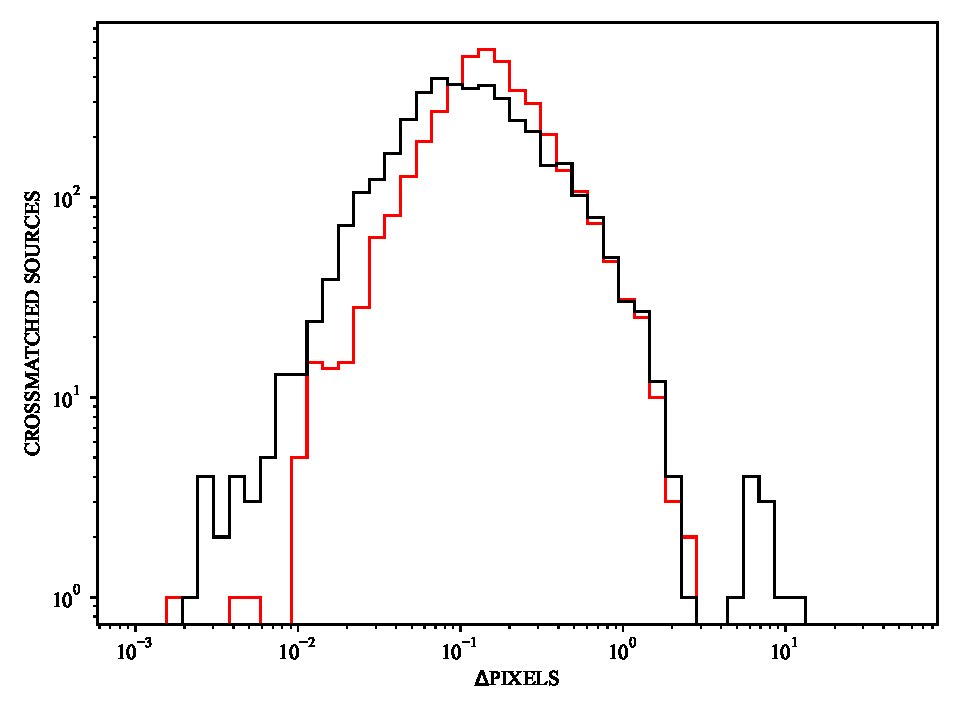
\includegraphics[width=\columnwidth]{Figure_4.pdf}
    \caption{Offset (in pixels) of cross-matched sources for the WCS solution calculated by \astrometrynet\ (red) and our refitted WCS solution (black) for a \ngts\ image centred around RA = $21^{h}$ 41', Dec = $-36^{\circ}$ 33' (Figure\,\ref{fig:Figure2}). }
    \label{fig:Figure_4}
\end{figure}


%We depend on a accurate world coordinate system (WCS) for each image to accurately position photometric apertures. 
We derive an initial WCS solution for each image using \astrometrynet\ \citep{2010AJ....139.1782L}. We use a  Simple Image Polynomial (SIP) of degree 3 to describe distortion across the image \citep{2005ASPC..347..491S}, and require \astrometrynet\ to re-fit polynomial coefficients to obtain a better solution. However, upon cross-matching suitable sources from TIC, we discovered that this solution inadequately compensates for distortion at the edges of the field of view, leading to drifts of up to several tens of pixels, as illustrated in the middle panel of Figure~\ref{fig:Figure2}.

Further improving on the \astrometrynet\ WCS solution required refining the SIP coefficients to more accurately represent the observed distortion across each frame. To accomplish this, we used TIC V8.0 to compile a catalogue of stars within the frame possessing valid Gaia DR2 IDs and magnitudes falling within the range $10<\rm T_{\rm mag} < 15$. The pixel positions of sources detected in the image (Section~\ref{sec:source_detection}) are converted to right ascension and declination using the initial WCS solution before being cross-matched with those from the TIC V8 catalogue. This comparison enabled the identification of additional distortion across the frame, prompting the re-fitting of the SIP coefficients to establish a more precise distortion model. The re-fitting considered measured brightness of sources to filter out sources with inconsistent brightnesses that may have been incorrectly crossmatched. This process is repeated until the median improvement changes by less than 1/100$^{th}$ of a pixel in both dimensions, or until 20 iterations have occurred\footnote{Most frames take $\sim$3-7 iterations.} (see right panel of Figure~\ref{fig:Figure2}). Figure~\ref{fig:Figure_4} illustrates the pixel offsets of cross-matched sources before and after the WCS solution re-fitting. Initially, with \astrometrynet\ alone, most stars exhibited offsets ranging from 1-10 pixels, a significant discrepancy given the $\sim3$ pixel point-spread function of a typical in-focus source observed with \ngts. Following the WCS solution re-fitting, the positions of most stars were calculated to within better than $\sim0.1$ pixels.




\section{Photometry}\label{sec:data_extraction}



\subsection{Target photometry catalogue}\label{sec:target_catalogue}

\begin{figure}
    \centering
    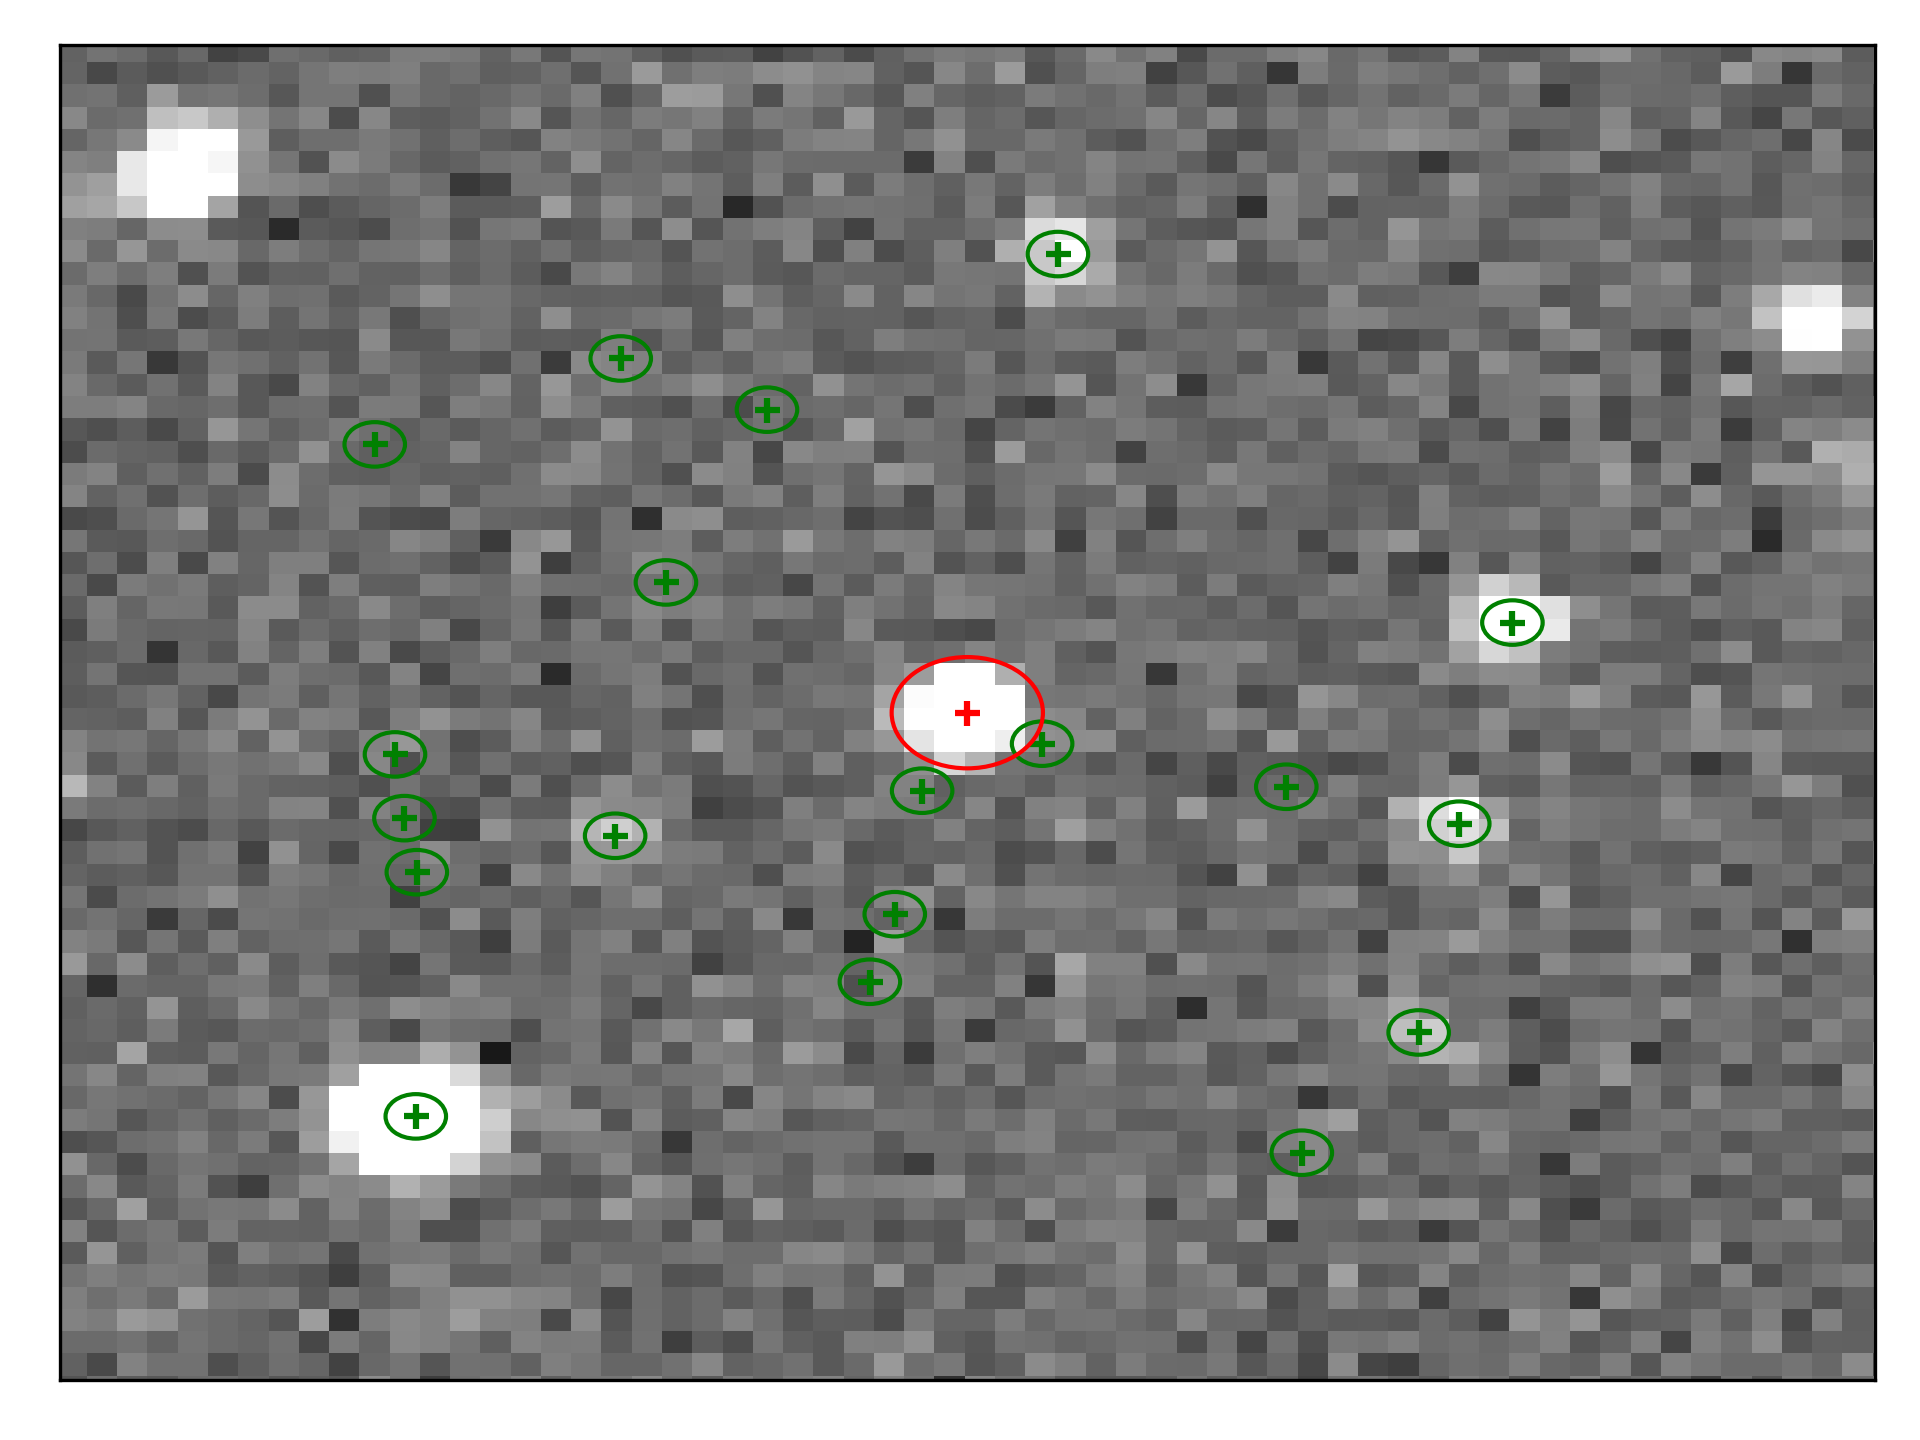
\includegraphics[width=\columnwidth]{NG0846-0223_804_IMAGE80420240926092124_blend_stars.png}
    \caption{A subset of the target photometry catalogue for TIC-1676693 showing the target (red) and stars near to the target, which could potentially introduce false-positive signals (green).}
    \label{fig:target_catalogue}
\end{figure}

Each autoguider reference image has its own target photometry catalogue which consists of all TIC V8.0 sources that fall on silicon. We extract photometry for all sources with \tess\ magnitudes smaller than 16. This limit may be relaxed if a fainter target is to be observed and comparison stars are needed. We include sources brighter than \tess\ magnitude 9 for focused observations despite saturation typically occurring for those sources. %The faint magnitude limit of 16 is often reduced for defocused observations to avoid extracting photometry for sources which are not detectable. This is done to avoid unnecessary digital storage. Photometry for each image is extracted using the target catalogue associated with its autoguider reference image. 

%The target photometry catalogue is curated from all TIC V8.0 sources common to all autoguider reference images for a given target and delineated into three distinct categories of stars. The first is the target star and therefore it is critical that it resides in TIC V8.0. The secondary group encompasses stars near to the target, which could potentially introduce false-positive signals (Figure\,\ref{fig:target_catalogue}). This subset is chosen to mitigate blend scenarios, particularly pertinent for targets originating from missions with coarser pixel scales (e.g. \tess). We inclusively select all stars located within 24 pixels (120") of the target or those brighter than the target within 48 pixels (240"). The third group comprises of comparison stars deemed suitable for conducting differential photometry alongside the target star.  Selection criteria encompass stars from the autoguider image catalogue positioned at least 200 pixels away from the auto-guider reference image edges, with TIC V8 entries denoting 'objType' as 'STAR' and 'lumclass' as 'DWARF'. Additionally, stars with calculated dilution values exceeding 5\% (Section~\ref{sec:dilution}) are excluded. Moreover, stars with \gaia\ BP-RP colors deviating by more than 1 magnitude from the target, if Tmag > 10, are omitted, with this threshold relaxed for brighter stars to broaden the pool of viable comparison stars. From the remaining comparison stars, a hierarchical ranking based on magnitude difference and pixel distance from the target is employed, with the latter weighted 500 times less than the former. This weighting scheme was empirically determined through iterative experimentation and the best 100 comparison stars become the comparison stars in the target photometry catalogue.



\subsection{Aperture photometry of each frame}

\begin{table}
    \centering

    \begin{tabular}{c|c}
    \hline
    \hline
    Image defocus [D; mm]& Aperture size [pixel] \\
    \hline
      $0\leq D < 0.1 $   & 3.0 \\
      $0.1\leq D < 0.2 $   & 3.5 \\
      $0.2\leq D < 0.3 $   & 4 \\
      $0.3\leq D < 0.4 $   & 4.5 \\
      $0.4\leq D < 0.5 $   & 5 \\
      $0.5\leq D < 0.6 $   & 6 \\
      $D > 0.6 $   & 7 \\
    \hline
    \end{tabular}
    \caption{Aperture sizes for photometry using various levels of defocus.}
    \label{tab:aperture_sizes}
\end{table}


We perform aperture photometry on the background-subtracted frame using the \textsc{sep sum\_circle} routine. We extract photometry for every star in the target photometry catalogue (Section \ref{sec:target_catalogue}) using an aperture suitable for the defocus of the image (Table~\ref{tab:aperture_sizes}). Aperture sizes were determined empirically from images taken at different defocus levels (Section~\ref{sec:source_detection} and Figure~\ref{fig:detection_kernels}). These are purposefully chosen to be 0.5 pixels too large to provide stability in instances where atmospheric seeing may deteriorate such that the point-spread function increases. Observations of fainter stars often benefit from a 2 pixel aperture as \ngts\ becomes background limited but we choose three pixels for similar reasons and to be consistent with the pipeline presented by \citep{2018MNRAS.475.4476W}. 

Apertures are centred from each frames improved WCS (Section~\ref{sec:WCS_solution}). The exact overlap between the aperture and pixels is used to determine the flux measurement and it's uncertainty given predetermined gain values for each camera. Additionally, we provide the maximum flux value derived from all pixels intersecting an aperture, to check that sources within the image are unsaturated and unaffected by nearby bright stars.

\subsection{Time conversions}

We use the \textsc{astropy} Python package \citep{astropy:2013,astropy:2018,astropy:2022} for time conversions within our analysis. For each image, we extract the modified Julian date (MJD) corresponding to the midpoint of exposure and subsequently compute the barycentric and heliocentric light travel times, thus deriving the Barycentric Julian Date (BJD) and Heliocentric Julian Date (HJD) at the midpoint of exposure for each object in the target photometry catalogue. The HJD values are reported in the UTC time scale, which reflects the current time at the zero-degree meridian, whereas the BJD values are reported in the barycentric dynamical time scale, governed by a clock positioned at the solar system barycenter. 
%Due to the extensive field of view of \ngts, the HJD and BJD corrections may exhibit variations of up to $\sim14$ minutes across each frame.


\subsection{Measuring the Point Spread Function}\label{sec:psf}

The Point Spread Function (PSF) offers valuable insights into observation quality. Temporal variations in the PSF can introduce systematic features in aperture photometry, potentially leading to spurious transit signals. We employ three distinct methods to measure the PSF. Firstly, we use the source detection algorithm within \textsc{sep}, which provides estimates for the full-width-half-maximum (FWHM) of each detected source in an image. For each frame, we compute the median FWHM value across all sources detected in the frame, as well as the median value derived from sources within the central 1024$\times$1024 pixels. Secondly, we measure the ellipsoidal parameters for sources within a super-sampled portion of the image. Each frame is partitioned into a $3\times 3$ grid, and sources within each grid cell are stacked and re-sampled to estimate representative values for the width, length, and orientation angle of an ellipse characterising the PSF. Lastly, we measure the FWHM from a rolling stack of the last 10 frames. Source extraction is performed using \textsc{sextractor} \citep{1996A&AS..117..393B}, and we report the mean FWHM value for each frame. These approaches collectively provide a complete characterisation of the PSF and aid in assessing and detrendeding observations.


% \subsection{Source dilution}\label{sec:dilution}

% The dilution for each source is determined by evaluating the mean point response function (PRF) across suitable stars in an image for each aperture (ranging from 2 to 10 pixels at intervals of 0.5 pixels). For a designated aperture size, we selectively consider sources from the autoguider image catalogue, ensuring a minimum separation of 7 pixels plus the aperture diameter from neighboring sources. We perform aperture photometry on each source radially (10 angular divisions from 0 to 10 pixel extent in 0.5 pixel increments) to measure the mean change in flux as an aperture moves away from the source (PRF). This is then averaged with the other suitable sources in the field to determine the mean, normalised PRF for the image. This normalised function elucidates the flux contribution of adjacent stars within a specified target aperture. This also adapts well for defocused images where the PSF moves towards a donut shape. We use all sources in TIC V8.0 which are on-silicon for the image and calculate a dilution value for each using the PRF for a given aperture, the \tess\ magnitude of the sources (assuming \tess\ has a similar transmission to \ngts), and the pixel distance to other sources in the frame. This results in a dilution for each aperture size (2-10\, pixels) which is used in Sections~\ref{sec:WCS_solution}\,\&\,\ref{sec:target_catalogue}.


\subsection{Centroiding}\label{sec:centroiding}

Accurate star positions on the CCD are pivotal for mitigating systematic errors stemming from non-uniform pixel response across an image. While \ngts\ has precise sub-pixel guiding, occasional systematic biases in aperture photometery from guiding issues can be seen. Centroid information is provided for each target to mitigate these issues. We report the pixel positions of each source utilising the improved WCS solution (Section~\ref{sec:WCS_solution}). We also report the re-centered pixel positions using the \textsc{sep winpos} function, which employs an iterative algorithm operating within a circular region surrounding each star. The window size is standardised to 9 pixels but is adjusted for defocused observations. %Finally, the flux-weighted average pixel position is reported, computed over a $10\times 10$ windowed region surrounding each source. 

%\subsection{Auxiliary information}

%We report a comprehensive amount of auxiliary information per image to ensure a thorough understanding of the observations. This supplementary data encompasses image identifiers, autoguider correction information, requested and actual telescope pointing coordinates, as well as technical details regarding the CCD and focuser. Information regarding the positions and illuminations of the Moon and Sun are presented, alongside pertinent meteorological data retrieved from weather stations, encompassing temperature, wind speed, atmospheric pressure, and humidity are included. A full list of these metrics is reported in \textbf{Table~\ref{X}}. 






\section{Data products}\label{sec:data_products}

\subsection{Low-level products}\label{sec:lowlevelproducts} 

% ACTION_335115_BJD.fits        ACTION_335115_PSF.fits
% ACTION_335115_FLAGS.fits      ACTION_335115_XC.fits
% ACTION_335115_FLUX_BKG.fits   ACTION_335115_X.fits
% ACTION_335115_FLUX_ERR.fits   ACTION_335115_YC.fits
% ACTION_335115_FLUX.fits       ACTION_335115_Y.fits
% ACTION_335115_IMAGELIST.fits

Low-level data products are archived in compressed (\textsc{bzip2}) FITS files are sorted into one folder per action, with one file dedicated to each data product per action, totalling 12 files per directory. The first file contains the Barycentric Julian date of mid observations for each source on the frame. This stored as a 2 dimensional fits file of type 32-bit integers, represented by the number of seconds elapsed since 2014-01-01T00:00:00. Three files store the flux measurements for each source - the flux in the optimal aperture, the formal errors on the flux measurements, and the flux measurement of the sky background. These are stored as a 2 dimensional fits file of type 32-bit floating point numbers. The WCS aperture positions (Section~\ref{sec:WCS_solution}) of each source are stored separately for both image dimensions. Similarly, the centroid positions (Section~\ref{sec:centroiding}) for each dimensions are also saved separately for each dimension. These are stored as a 2 dimensional fits file of type 16-bit unsigned integers. Finally, an observation summary file is made for each action which contains a fits table in extension 1. This provides auxiliary information about the observations (e.g. airmass, humidity, Moon angle and brightness). 


% \subsection{Optimal aperture}\label{sec:dataproducts:optimal_aperture}

% The selection of an optimal aperture size is important for achieving precise photometry. An aperture that is excessively small, failing to fully encompass the PSF of a source, leads to the exclusion of measurable flux and results in red noise correlated with atmospheric conditions, airmass, and centroiding offsets. Conversely, an overly large aperture incorporates excessive background noise, reducing the contrast of the photometric measurements, and risks contamination from neighbouring stars. \ngts\ has an undersampled point-spread function with a full-width half maximum of around 2 pixels and a 3-pixel radius aperture has been traditionally used for in-focus observations. However, we found that a 2-pixel aperture is advantageous under favourable observing conditions or within densely populated fields. Furthermore, defocused observations require a larger aperture to adequately encapsulate the broader, donut-shaped point-spread functions. In the final lightcurve product (Section~\ref{sec:final_product}) we report photometry only for the optimal aperture and so significant care is take to ensure the best aperture is selected.

% We find the optimal aperture by stacking all available data together. For each night, the measured target flux in all apertures is detrended with a third degree polynomial against time to remove correlated noise which may be astrophysical or caused by observing strategy/conditions. The aperture yielding the lowest measured standard deviation is identified as the optimal choice and typically falls within radii ranging from 2 to 4 pixels for focused observations. The median aperture across all nights is selected as the optimal aperture, with care taken to exclude poor quality observations. This can be repeated as new data becomes available under improved weather conditions. Alternatively, it can be conducted on a higher-quality comparison star if the target source proves unsuitable (e.g. blended or highly variable). The aperture selection is intertwined with comparison star rejection and more details can be found in Section~\ref{sec:detrended_lc}.


\subsection{Detrendeding observations}\label{sec:detrended_lc}

The change in airmass during a night stands as one of many prominent systematic trends impacting flux measurements obtained from ground-based observatories. Photometry of many targets during a sequence of observations will show similar trends and can produce a common set of basis vectors that are fit to photometric measurements to detrend the data. We use the \textsc{sysrem} algorithm \citep{2007ASPC..366..119M} which has proven performance in wide angle photometric missions from the ground (e.g. \wasp and \ngts).

Photometry is first grouped by autoguider reference image as photometry derived from each reference image has unique offsets and systematics. We flag photometric data points which are affected by the VLT laser and those more than 7-$\sigma$ from the median flux for a given source. We then perform a coarse decorrelation with airmass and CCD positions to remove prominent trends, while simultaneously down-weighting variable stars and cloudy images. We then use the \textsc{sysrem} algorithm to remove up to 5 of the most prominent co-trending basis vectors from raw photometric measurements of each target. Flagged data points do not contribute to the measurements of basis vectors. The result is a 2 dimensional fits file of type 32-bit floating point numbers which contains the detrended flux. An summary file for the \textsc{sysrem} algorithm is created which contains a fits table in extension 1. This contains information regarding the basis vectors, which stars where used to create the basis vectors, and measurements of the variance across an image (\textsc{sigma\_xs}) and the photometric zero point - the latter two are important for excluding measurements affected by clouds. 
 

We found through extensive testing that this works robustly on photometry grouped by autoguider reference image, but very occasionally fails to detrend individual nights for unknown reasons.  To overcome this, we also run a coarse decorrelations and \textsc{sysrem} on each individual action. The benefits of this are two-fold. First, it provides alternative detrending should the first implementation of coarse decorrelations and \textsc{sysrem} fail. Second, systematic trends may be more robustly captured for individual nights and provide better detrended data, but photometric offsets amongst actions of the same reference image will not be preserved (see Section~\ref{sec:aligning_photometry}). 




% The change in airmass during a night stands as one of a few prominent systematic trends impacting flux measurements obtained from ground-based observatories. The comparison stars extracted offer a way to mitigate these trends, as such features are common to both the target flux and the comparison star flux. This pipeline creates a master comparison star by summing up the flux measurements from all suitable comparison stars (Section~\ref{QL:target_catalogue}). The target flux measurements and respective errors are then divided by the master comparison star fluxes to remove the effect of the atmosphere. 

% Some comparison stars show deep eclipses or excessive astrophysical noise and so only a subset of comparison stars are typically used. Unlike Section~\ref{sec:dataproducts:optimal_aperture}, we identify bad comparison stars by stacking all available data together, ensuring that photometric offsets from different cameras are accounted for (Section~\ref{sec:aligning_photometry}). First, plot the maximum recorded flux measurement within 10 pixels for each comparison star against Tmag and exclude stars that exceed 3-$\sigma$ from the mean determined through a polynomial of order 3. This excludes comparison stars affected by diffraction spikes or saturation trails of nearby bright stars. This is then repeated using the median flux for each comparison star using the optimal aperture to exclude stars which have excessive flux measurements likely due to blending or nearby bright stars. We then repeat this with the standard deviation of maximum flux recorded within the optimal aperture to ensure no bright star features may occasionally move into the optimal aperture. 

% We further look to exclude comparison stars by inspecting their properties on a per-action basis. We calculate the standard deviation of each comparison stars flux for each action by detrending against time using a polynomial of order 3. We calculate the sum of these standard deviations over each action and compare that to the stars Tmag to exclude stars that have excessive variability on long timescales ($>1$\,day). This is a more subtle test of astrophysical variability and is is efficient at detecting comparison stars with small-amplitude stellar variability. The remaining comparison stars are used to create a master comparison star.

% In practice, determining the optimal aperture (Section~\ref{sec:dataproducts:optimal_aperture}) and rejecting comparison stars are intertwined as one depends on the other. We first select an optimal aperture based purely on the defocus of these observations (3 pixels for focused observations up to 7 pixels for 0.6\,mm defocus) which was determined empirically. Comparison stars are rejected as outlined above and then the standard deviation of each comparison stars flux for each action is summed for a given night to poor-quality nights. These are then rejected and the remaining data used to select the optimal aperture as outlined in Section~\ref{sec:dataproducts:optimal_aperture}. The comparison star rejection is then repeated, poor quality nights rejected, and the optimal aperture measured again. If the optimal aperture remains the same as the previous iteration, we conclude the process as complete. 




\subsection{Aligning photometry from different cameras}\label{sec:aligning_photometry}

Some targets are observed with multiple telescopes at the same time, or are observed with different telescopes at various points in a photometric campaign. Each camera exhibits a distinct response to observations of the same fields and variations in photometric zero-points are inevitable and need to be accounted for. For multicamera observations of transits intended for publication, it is best to treat each cameras dataset as unique and fit unique photometric zero-point alongside the transit model. For photometric monitoring campaigns which used multiple telescopes, but with only one telescope in operation at any given time, it is necessary to determine the photometric offsets between observations. In practice, each dataset that uses a distinct autoguider reference image requires a photometric offset to be calculated as there can be offsets even when observed on the same camera.\footnote{Autoguider reference images may occasionally change due to presence of clouds/laser/satellites in the initial image, or after a camera/telescope hardware repair.}

The quick-look pipeline provides photometric zero-points offsets for each autoguider image by looking at the median flux measurements for each dataset across both individual nights and the entire dataset. The autoguider image with the most associated data points becomes the image from which the photometric zero-points of all other autoguider images are aligned to. First, we search all nights where the reference image observed simultaneously with other autoguider images. By comparing the median detrended target flux measurements for those observation we can directly calculate the photometric offsets for those autoguider images. We repeat this process until the photometric offsets are calculated for all autoguider images, there are no more overlapping observations such that any more photometric offsets can be measured. In those cases, we calculated the photometric offsets by comparing the median of the detrended target flux to to that from the reference auotguider image. Care should be taken to when stacking data based upon these offsets and each subset of data from an individual autoguider image should be treated as unique and separate datasets where possible.


\subsection{Final product}\label{sec:final_product}


\begin{table}
    \centering
    \begin{tabular}{c|l|l}
    \hline
    \hline
    Column & Data type & Description \\
    \hline
    TIC\_id & INT & The TIC ID\\
    Gaia\_id & INT & The Gaia ID\\
    % phot\_type & INT & Target type\\
    % metric & FLOAT & The metric used to select comparison\\
    % &              & stars \\
    ra\_deg & FLOAT & The J2000 right ascension [degrees]\\
    dec\_deg & FLOAT & The J2000 declination [degrees]\\
    pmRA & FLOAT & The proper motion in right ascension\\
    &&[mas\,yr$^{-1}$]\\
    pmDEC & FLOAT & The proper motion in declination \\
    &&[mas\,yr$^{-1}$]\\
    $i$ mag & FLOAT & The sloan $i$ magnitude\\
    GAIAmag & FLOAT & The \gaia\ magnitude\\
    Jmag & FLOAT & The two mass J magnitude\\
    objType & STRING & The Object type according\\
    &&to TIC V8.0\\
    lumclass & STRING & The luminosity classification according\\
    &&to TIC V8.0\\
    on\_chip & INT & If the source is on-silicon or  not.\\
    ra\_deg\_corr & FLOAT & The J2000 right ascension [degrees]\\
    &&corrected for proper motion\\
    dec\_deg\_corr & FLOAT & The J2000 declination [degrees] corrected\\
    &&for proper motion\\
    \hline
    \end{tabular}
    \caption{Names, data types, and descriptions of columns in the first extension of the final product (target photometry catalogue).}
    \label{tab:final_product_cols_tab1}
\end{table}

\begin{table}
    \centering
    \begin{tabular}{c|l|l}
    \hline
    \hline
    Column & Data type & Description \\
    \hline
    action\_id & INT & The action ID\\
    camera\_id & INT & The camera ID\\
    night & STR & The night of observation\\
    action\_type & STR & The type of observation\\
    actual\_start\_utc & DATETIME & The start of the observations. \\
    actual\_end\_utc & DATETIME & The end of the observations. \\
    status & STR & Whether it completed, failed to start, \\
    & & or aborted. \\
    field & STR & The field name [NGXXXX-YY]. \\
    campaign & STR & The observing campaign name. \\
    autoguided & STR & Whether autoguiding was used. \\
    ref\_image\_id & INT & The reference image used to guide\\
    & & tracking. \\
    gain\_idx & INT & The gain setting index. \\
    num\_images & INT & The number of images obtained \\
    mean\_moon\_dist & FLOAT & The mean moon distance in degrees. \\
    args & STR & Additional arguments for the\\
    & & observation. \\
    num\_extracted & INT & The number of images reduced. \\
    \hline
    \end{tabular}
    \caption{Names, data types, and descriptions of columns in the table in fits extension 2 of the final photometry file (observation summary log).}
    \label{tab:final_product_cols_tab2}
\end{table}




\begin{table}
    \centering
    \begin{tabular}{c|l|l}
    \hline
    \hline
    Column & Data type & Description \\
    \hline
    SIGMA\_XS\_ACTIONXXXXXX & float & A measure of the variance across each measured source in action XXXXXX.\\
    CI\_ACTIONXXXXXX & float & ASK RICHARD\\
    IS\_STD\_ACTIONXXXXXX & int & A flag to measure if a star was used as a standard to derive basis vectors for \textsc{sysrem}.\\
    \hline
    \end{tabular}
    \caption{Names, data types, and descriptions of columns in the table in fits extension 3 of the final photometry file (action \textsc{sysrem} information).}
    \label{tab:final_product_cols_tab3}
\end{table}

\begin{table}
    \centering
    \begin{tabular}{c|l|l}
    \hline
    \hline
    Column & Data type & Description \\
    \hline
    FLAGS & INT & Photometric flag set vefore the pipeline.\\
    IMAGE\_ID & INT & The image ID.\\
    NIGHT & INT & The night of the observation represented as YYYYMMDD.\\
    AIRMASS & FLOAT & The airmass of the image at the commanded RA and Dec.\\
    TEL\_HA & FLOAT & The hour angle [degrees] at the commanded RA and Dec.\\
    reduced & bool & Boleon describing if the image was reduced or not.\\
    \hline
    \end{tabular}
    \caption{Names, data types, and descriptions of columns in the table in fits extension 4 of the final photometry file (image information).}
    \label{tab:final_product_cols_tab4}
\end{table}




\begin{table*}
    \centering
    \begin{tabular}{c|l|l}
    \hline\hline
    Column & Data type & Description \\
    \hline
    BJD & DOUBLE & The barycentric julian date. \\
    BJD\_SHORT & DOUBLE & The barycentric julian date with gaps removed. \\
    X & DOUBLE & The x-coordinate of the target from the re-fittted world-coordinate system \\
    XC & DOUBLE & The x coordinate of the target centroid from \textsc{sep}.\\
    Y & DOUBLE & The y-coordinate of the target from the re-fittted world-coordinate system \\
    YC & DOUBLE & The y coordinate of the target centroid from \textsc{sep}.\\
    FLAGS\_1 & INT & Flags set by the per-action reduction. \\
    PFSSEP & DOUBLE & The PSF width in the centre of the frame from \textsc{sep}.\\
    PFSTOM & DOUBLE & The PSF width in the center third of the frame calculated from super-sampled PSFs. \\
    PFSRICH & DOUBLE &  The PSF width calculated from a rolling stack of the last 10 frames. \\
    FLUX & DOUBLE & The target flux measured with the optimal aperture. \\
    FLUX\_SYSREM & DOUBLE & The target flux detrended with \textsc{sysrem} for all observations. \\
    FLUX\_SYSREM\_ACTION & DOUBLE & The target flux detrended with \textsc{sysrem} for the action. \\
    FLUX\_ERR & DOUBLE & The error on the target flux. \\
    FLUX\_BKG & DOUBLE & The flux of the sky background. \\
    SIGMA\_XS & FLOAT & A measure of the variance across the frame of the image. \\
    ZERO\_POINT & FLOAT & A measure of the photometric zero-point for the frame.\\
    AJ & float[] & ASK RICHARD\\
    NIGHT\_IDX & INT & Unique integer for each night of observations. \\
    FLAGS\_2 & INT & Flags set after \textsc{sysrem}. \\
    ZP\_FIT & FLOAT & The fitted zero-point.\\
    EXT\_XSLOPE & FLOAT & ASK RICHARD\\
    EXT\_YSLOPE & FLOAT & ASK RICHARD\\


    SIGMA\_XS\_ACTION & FLOAT & A measure of the variance across the frame of the image for each action. \\
    ZERO\_POINT\_ACTION  & FLOAT & A measure of the photometric zero-point for the frame for each action.\\
    AJ\_ACTION  & float[] & ASK RICHARD\\
    NIGHT\_IDX\_ACTION  & INT & Unique integer for each night of observations for each action. \\
    FLAGS\_ACTION  & INT & Flags set after \textsc{sysrem} for each action for each action. \\
    ZP\_FIT\_ACTION  & FLOAT & The fitted zero-point  for each action.\\
    EXT\_XSLOPE\_ACTION  & FLOAT & ASK RICHARD\\
    EXT\_YSLOPE\_ACTION  & FLOAT & ASK RICHARD\\
    \hline
    \end{tabular}
    \caption{Names, data types, and descriptions of columns in extension 5 (photometry) of the final product.}
    \label{tab:final_product_cols_tab5}
\end{table*}

Low-level products from the per-action photometry (Section~\ref{sec:lowlevelproducts}) are available to use, but a final product is provided in the form of a single fits file containing five table extensions. 

Extension one contains the photometric catalogue for which photometry was extracted. This table, describe in Table\,\ref{tab:final_product_cols_tab1}, contains a subset of columns found in TIC V8.0 for use in the pipeline. Three additional columns were created: ra\_deg\_corr and dec\_deg\_corr provide the coordinates of each source corrected for proper motion at the time the autoguider reference image was obtained, and on\_chip which describes if the source was imaged on the autoguider reference image. Throughout the running of the reduction pipeline, this catalogue is much more extensive adding sources with $Tmag>16$ and those that are not imaged on the autoguider image to assist in WCS solutions. Here we only provide sources on silicon (on\_chip=1) and $Tmag<16$ (of which photometry was extracted for).

Extension two contains an observation summary log for the target. This contains information about the individual actions including the camera identification number, the night, the bounding times of the observation for each action, whether it terminated early or completed successfully, the associated reference image ID, the camera gain setting, the number of images obtained, and the mean moon distance for the action in degrees. These columns are summarised in Table~\ref{tab:final_product_cols_tab2}. 

Extension three contains relevant columns from the \textsc{sysrem} detrending of individual actions. This includes the measure of variance across the frame -- \textsc{sigma\_xs}, the correlation coefficients, and whether the star was used a standard to derive basis vectors. These three columns are repeated for each action and is summarised in Table\,\ref{tab:final_product_cols_tab3}.

Extension four contains information on each individual image reduced. Each row corrosponds to an image and includes the image ID, image flags not set by the pipeline, the night of observation, the airmass of the image (at the commanded RA and Dec), the telescope hour angle in degrees), and weather the image was reduced. These columns are summarised in Table\,\ref{tab:final_product_cols_tab4}.

Extension five contains photometry information for a given target. This includes BJD, WCS positions, centroid positions,   photometric flags, PSF metrics, flux measurements, and \textsc{sysrem} outputs for both the individual actions and all the actions together. These columns are summarised in Table\,\ref{tab:final_product_cols_tab5}.


\section{Photometric performance and examples}

\begin{figure}
    \centering
    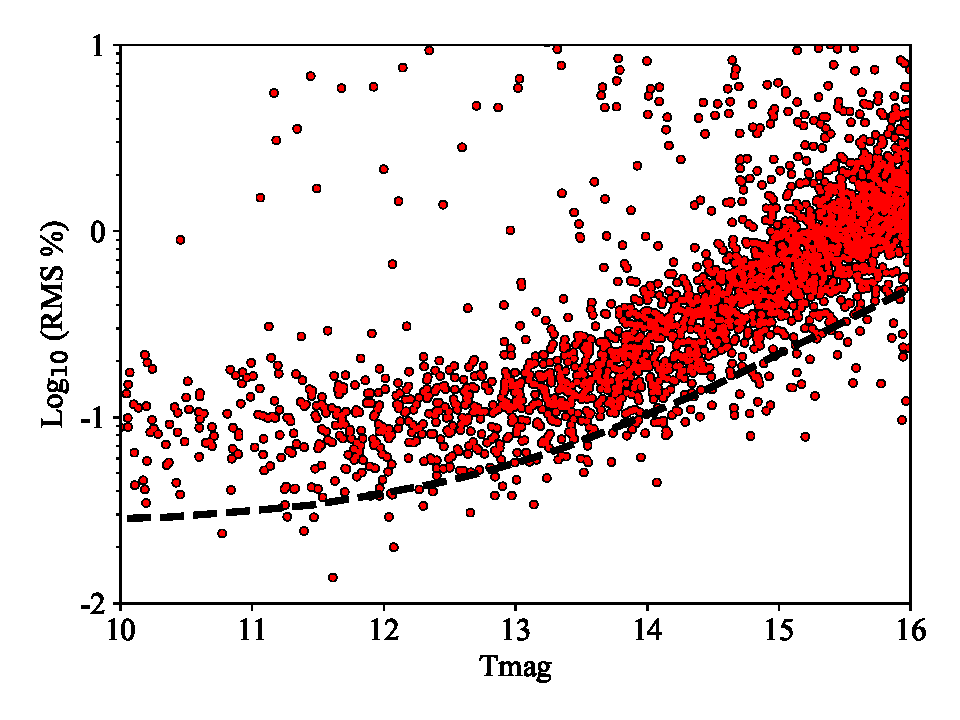
\includegraphics[width=\columnwidth]{PAOPhot2_performance.pdf}
    \caption{Noise for 1\,hour exposure time of 333 objects observed with one \ngts\ telescope at Paranal using the quick-look pipeline (black and red). We choose only targets that were not known to be transiting or eclipsing, and exclude multicamera observations. The schematic noise model for a dark sky in I-band ($\approx \rm T_{\rm mag}$) from \citet{2018MNRAS.475.4476W} is shown for reference (black-line).  }
    \label{fig:paophot2_performance}
\end{figure}

In Figure~\ref{fig:paophot2_performance} we show the photometric performance for 3130 objects observed with \ngts\ and processed with the quick-look pipeline. These were focused observations taken to recover an exoplanet transit signal for a star in the center of the field. We find that a 1-hour exposure can yield a typical photometric noise of $\sim$0.01\,\% below T$_{\rm mag}$ 14 and is competitive with the simulated noise model for a single \ngts\ telescope from \citet{2018MNRAS.475.4476W}. Other publications have extensively tested the noise performance of defocused observations and those with multiple cameras \citep[e.g.][]{2020MNRAS.494.5872B,OBrien21} and so we do not show that here.

\begin{figure}
    \centering
    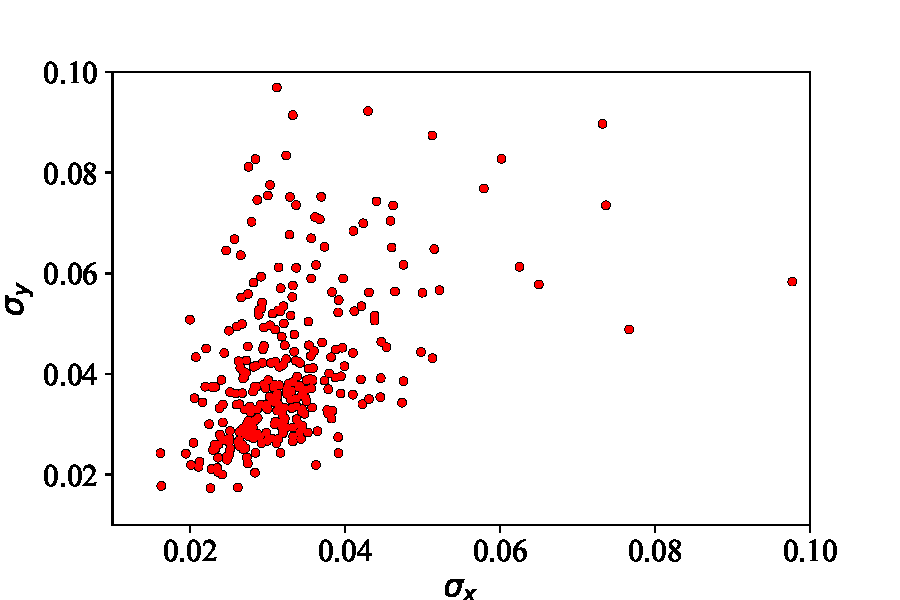
\includegraphics[width=\columnwidth]{PAOPhot2_performance_centroiding.pdf}
    \caption{Tracking performance for 333 objects observed with one NGTS telescope at Paranal using the quick-look pipeline (black and red). Each axis is the standard deviation of pixel coordinates for the target against those in the reference image. We choose only targets that were not known to be transiting or eclipsing, and exclude multicamera observations.  }
    \label{fig:paophot2_performance_centroiding}
\end{figure}

The photometric stability of \ngts\ is due in-part to the success of the autoguiding system. Through the use of reference images and the \textsc{donuts} algorithm \citep{2013PASP..125..548M}, each \ngts\ telescope is capable of keeping a target within the same pixel throughout a given night and subsequent nights. Figure~\ref{fig:paophot2_performance_centroiding} shows that \ngts\ tracks the target star to better than 1/10$^{th}$ of pixel, during the night and in subsequent nights. Doing so mitigates potential sources of red-noise from the camera and yields stable photometric measurements across multiple nights.

Examples of \ngts\ photometry can be found numerous publications\footnote{\href{ngtransits.org}{ngtransits.org}} and data reduced with the quick-look pipeline has been pivotal in photometric monitoring of planet hosts \citep[e.g. WASP-39; ][]{2023Natur.614..653A}, precise multicamera transits \citep[e.g. ][]{2020MNRAS.494.5872B,2020Natur.583...39A,2022MNRAS.514.1606B}, and determining the orbital period of \tess\ single-transit planets \citep{2020ApJ...898L..11G}. Observations for a variety of science programs can be requested\footnote{contact p.j.wheatley@warwick.ac.uk for more information.} and data provided in a timely fashion.





%section{Differences from the main pipeline}

%The pipeline described here has been designed to optimise photometry of a specific target and shares some similarities with the current form of the main \ngts\ pipeline used to search for planet candidates \citep[Described in ][]{2018MNRAS.475.4476W}. One major difference in pre-processing is that the main pipeline creates and uses master dark, bias, and flat frames to create reduced science frames. This pipeline does not implement this as the quality of the photometric measurements are only marginally improved. Both pipelines remove the over-scan region, estimate the sky background as described in Section~\ref{sec:backrgound}, and detect the VLT laser as described in Section~\ref{sec:laser_detection}. \textbf{However, the main pipeline makes no attempt to identify satellites in a given frame.} Finally, both pipelines use the method described in Section~\ref{sec:WCS_solution} to determine and improve the world coordinate system solution for each image. 

%The photometry catalogue differs significantly as each pipeline has separate objectives. The main \ngts\ pipeline aims to discover transiting planets around all suitable stars in the frame while this pipeline is optimised for specific targets. Since 2022, the photometry catalogue for the main pipeline has been list-driven (TIC V8) and includes all stars brighter than  $\rm T_{\rm mag}<16$ and those suitable for auxiliary science (young stars, white dwarfs, etc). The main pipeline extracts photometry for many more objects but the structure of the low-level products in this pipeline (Section~\ref{sec:lowlevelproducts}) is very similar to those from the main pipeline. Detrending in the main pipeline is different and uses the \textsc{sysrem} algorithm \citep{2007ASPC..366..119M} to remove up to 5 of the most prominent co-trending basis vectors from raw photometric measurements of each target.  


\section{Conclusions}\label{sec:conclusion}

In this paper we present the \ngts\ high-precision targeted mode of operations and the subsequent pipeline to reduce observations. These observations involve imaging known transiting exoplanets  with one or more cameras \citep[e.g.][]{2020MNRAS.494.5872B,2020Natur.583...39A,2022MNRAS.514.1606B,2022MNRAS.510.5464K,2024A&A...688A.211L},  photometric monitoring to recover transits of long-period planets with a single camera \citep[e.g.][]{2020ApJ...898L..11G,2024MNRAS.532.1444G}, constraining stellar activity \citep[e.g.][]{2023Natur.614..653A}, or supporting observation on other by other observatories \citep{2022MNRAS.516..298D,2023MNRAS.522.4499D}.

We describe the targeted mode of operations in detail, the capabilities of the observatory, and complimentary projects. Image processing is described in Section~\ref{sec:preprocessing}, including detecting the laser from the VLT's 4 laser guide star facility, detecting satellites, sky background estimation, and source detection. We also describe our approach to obtain and improve the WCS solution through iteratively crossmatching sources and re-fitting the SIP coefficients. We find our improved WCS solution is typically better to 0.1 pixels at the edge of the frame. 

This paper describes how we generate a target photometry catalogue for a given target and how we perform aperture photometry on each frame. We describe auxiliary measurements such as the point-spread function, centroiding, dilution values using the PRF, and time conversions. The data products for the pipeline are described in Sections~\ref{sec:lowlevelproducts} \& \ref{sec:final_product}. The \ngts\ targeted mode of operations and the pipeline described here is capable of producing publication-quality light-curves for individual targets that typically exceed the predicted noise model for \ngts (Figure~\ref{fig:ngts_precision}). This is due in-part to the observational strategy, pipeline, and exceptional optical design and stability.





\section*{Acknowledgements}

This work is based on data collected under the NGTS project at the ESO Paranal Observatory. The NGTS facility is operated by a consortium institutes with support from the UK Science and Technology Facilities Council (STFC) under projects ST/M001962/1, ST/S002642/1 and ST/W003163/1.
The contributions at the University of Warwick by SG, DB, PJW, and RGW have been supported by STFC through consolidated grants ST/P000495/1, ST/T000406/1 and ST/X001121/1.
This work made use of Astropy:\footnote{http://www.astropy.org} a community-developed core Python package and an ecosystem of tools and resources for astronomy \citep{astropy:2013, astropy:2018, astropy:2022}.

%%%%%%%%%%%%%%%%%%%%%%%%%%%%%%%%%%%%%%%%%%%%%%%%%%
\section*{Data Availability}

Data used in this work are available upon request. 




%%%%%%%%%%%%%%%%%%%% REFERENCES %%%%%%%%%%%%%%%%%%

% The best way to enter references is to use BibTeX:

%\bibliographystyle{rasti}
\bibliographystyle{mnras}

\bibliography{paper} % if your bibtex file is called example.bib

% Alternatively you could enter them by hand, like this:
% This method is tedious and prone to error if you have lots of references
%\begin{thebibliography}{99}
%\bibitem[\protect\citeauthoryear{Author}{2012}]{Author2012}
%Author A.~N., 2013, Journal of Improbable Astronomy, 1, 1
%\bibitem[\protect\citeauthoryear{Others}{2013}]{Others2013}
%Others S., 2012, Journal of Interesting Stuff, 17, 198
%\end{thebibliography}

%%%%%%%%%%%%%%%%%%%%%%%%%%%%%%%%%%%%%%%%%%%%%%%%%%

%%%%%%%%%%%%%%%%% APPENDICES %%%%%%%%%%%%%%%%%%%%%

\appendix

\section{Some extra material}

If you want to present additional material which would interrupt the flow of the main paper,
it can be placed in an Appendix which appears after the list of references.

%%%%%%%%%%%%%%%%%%%%%%%%%%%%%%%%%%%%%%%%%%%%%%%%%%


% Don't change these lines
\bsp	% typesetting comment
\label{lastpage}
\end{document}

% End of rasti_template.tex
